\chapter{可行迭代}
\label{chap:feasible-iterations}

把一单位预算分给三个项目，$x_i$是第$i$个项目分到的比例。比例不能为负，三者之和必须为一，所以允许的分配构成一个三角形。假设方案的代价是下面的二次函数，三个系数表示各项目偏离理想份额时代价增长的快慢：
\begin{equation}
 f(\bm{x})=\frac12\Bigl[(x_1-1)^2+4\bigl(x_2-\tfrac58\bigr)^2+2x_3^2\Bigr].
 \label{eq:feas-running}
\end{equation}

理想份额$(1,\tfrac58,0)$的和是$\tfrac{13}{8}$，预算不够，所以约束一定起作用。梯度和Hessian分别是
\[
 \nabla f(\bm{x})=\bigl(x_1-1,\;4x_2-\tfrac52,\;2x_3\bigr),
 \qquad
 \nabla^2f=\operatorname{diag}(1,4,2).
\]
于是光滑常数$L=4$，强凸常数$\mu=1$。

这个问题的解是$\bm{x}^\star=(\tfrac12,\tfrac12,0)$，最优值$f^\star=\tfrac{5}{32}$，第~\ref{sec:feas-pgd-residual}节会验证这一点。图~\ref{fig:feas-running-simplex}把三维空间里的这个三角形摊平画出，三个顶点是把全部预算给一个项目的方案。解落在底边上，第三个项目分不到预算。

\begin{BookInlineFigure}
  \centering
  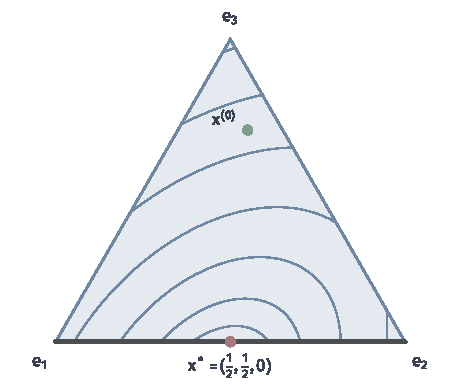
\includegraphics[width=78mm]{figures/05-optimization/06-constrained-optimization/matplotlib/feas-running-simplex/figure.pdf}
  \caption{贯穿全章的资源分配例。浅蓝三角形是$\{\bm{x}\geq\bm{0},\,x_1+x_2+x_3=1\}$，顶点$\bm{e}_i$是第$i$个坐标为$1$的单位向量。蓝线是式~\eqref{eq:feas-running}在三角形上的等高线，绿点是起点$(0.1,0.2,0.7)$，红点是最优解，深灰粗线是活动约束$x_3=0$所在的边。}
  \label{fig:feas-running-simplex}
\end{BookInlineFigure}

梯度下降的一步会把点带出三角形：坐标和不再是一，某些坐标可能变负。这一章研究的问题是：怎样让每个迭代点都满足原约束，保持可行又要付出多少计算？

第~\ref{sec:feas-updates}节先比较可以调用的几种运算。随后三节留在闭凸集合上，用同一个预算问题比较三种走法：先走再拉回最近点，朝线性模型的最优顶点靠拢，以及换一把更贴合比例结构的尺子。第~\ref{sec:feas-grg}节转向圆周这样的弯曲约束，这时连接两个可行点的线段不再可行，需要局部消元并解方程回到约束上。最后一节说明这些方法在什么前提下才能放在一起比较，以及算完之后应该报告什么。

\section{可行集合上的更新}
\label{sec:feas-updates}

设$\bm{C}\subseteq\mathbb{R}^n$是非空闭凸集，$f$在包含$\bm{C}$的开集上可微，要解
\begin{equation}
 \min_{\bm{x}\in\bm{C}}f(\bm{x}).
 \label{eq:feas-problem}
\end{equation}
有了当前可行点和它的梯度，还需要关于$\bm{C}$的什么额外运算，才能算出下一个可行点？

\paragraph{三种集合运算}
梯度只描述目标，对集合一无所知。把集合的信息送进更新，最常见的有三个渠道，它们分别回答三个不同的问题。

第一种是\term{投影}（projection）：给定任意点$\bm{z}$，问$\bm{C}$中离它最近的点在哪里。第二种是线性最小化：给定方向$\bm{g}$，问$\bm{C}$中沿$-\bm{g}$走得最远的点在哪里，也就是求$\min_{\bm{s}\in\bm{C}}\langle\bm{g},\bm{s}\rangle$。第三种是用一个由集合结构决定的非欧氏尺度求“最近点”，第~\ref{sec:feas-mirror}节会定义这把尺子。

图~\ref{fig:feas-three-oracles}在预算三角形上取同一个当前点，把三种运算画在一起。投影梯度先离开集合再回来，新点落在边界上；条件梯度沿当前点与顶点的线段移动，新点是两个可行点的组合；镜像更新走一条弯曲的路径，靠近边界时自动减速。

\begin{BookInlineFigure}
  \centering
  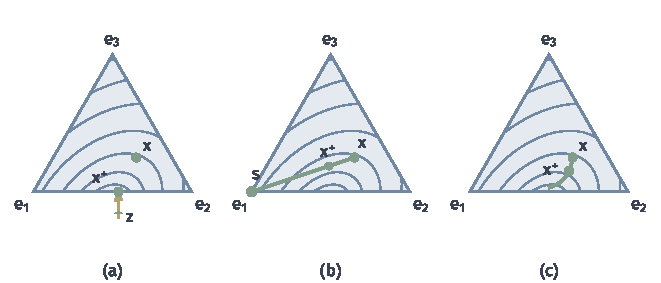
\includegraphics[width=112mm]{figures/05-optimization/06-constrained-optimization/matplotlib/feas-three-oracles/figure.pdf}
  \caption{预算三角形上从同一点$\bm{x}=(0.225,0.525,0.25)$出发的三种更新，为看清位移取较大的步长$\alpha=0.6$。(a)投影梯度：绿色箭头是平面内的梯度步，到达三角形外的空心点$\bm{z}$，黄色虚线把它拉回最近点$\bm{x}^{+}$。(b)条件梯度：线性模型在顶点$\bm{s}$处最优，新点是线段上的一点，图中取组合系数$0.25$。(c)镜像更新：绿线是步长从$0$增大时新点的轨迹，它始终留在三角形内部。}
  \label{fig:feas-three-oracles}
\end{BookInlineFigure}

\paragraph{凸性给了什么，没给什么}
$\bm{C}$凸意味着两个可行点之间的线段仍然可行。这保证条件梯度的组合可行，也保证投影存在唯一。图~\ref{fig:feas-segment-vs-curve}(a)画的就是这种情形。

凸性并不保证子问题便宜。在几千个一般线性不等式定义的多面体上，投影本身就是一个二次规划。在迹为一的半正定矩阵集合上，投影需要完整的特征分解，线性最小化却只需要一个最小特征向量。在单纯形上，投影和线性最小化都很便宜。所以选哪种方法，要先问手上的集合支持哪种运算。

\begin{BookInlineFigure}
  \centering
  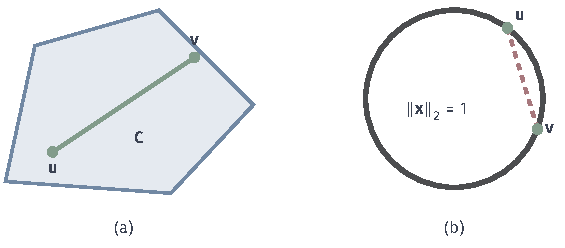
\includegraphics[width=95.75mm]{figures/05-optimization/06-constrained-optimization/tikz/feas-segment-vs-curve/figure.pdf}
  \caption{两种可行集合的差别。(a)凸集$\bm{C}$中两点$\bm{u},\bm{v}$的连线（绿色）留在集合内。(b)圆周$\lVert\bm{x}\rVert_2=1$上两点的连线（红色虚线）除端点外全部不可行，沿直线走的任何一步都要再回到圆周上。}
  \label{fig:feas-segment-vs-curve}
\end{BookInlineFigure}

\paragraph{各节使用的假设}
表~\ref{tab:feas-assumptions}列出后面各节的前提。前三行共用“集合是闭凸的”这一点，具体要求仍各不相同：条件梯度要求集合紧，否则线性子问题可能无解；镜像下降还要求势函数与集合匹配。

\begin{BookInlineTable}
  \centering
  \caption{本章各方法使用的集合、额外运算与评价量。}
  \label{tab:feas-assumptions}
  \begin{tabular}{llll}
   \toprule
   方法 & 集合 & 额外运算 & 评价量\\
   \midrule
   投影梯度 & 非空闭凸 & 欧氏投影 & 目标差、残差\\
   条件梯度 & 非空紧凸 & 线性最小化 & 目标差、间隙\\
   镜像下降 & 闭凸，配势函数 & Bregman子问题 & 平均点目标差\\
   GRG & 光滑等式加界 & 解方程 & 约束与KKT残差\\
   \bottomrule
  \end{tabular}
\end{BookInlineTable}

最后一行与前三行性质不同。图~\ref{fig:feas-segment-vs-curve}(b)的圆周不是凸集，前三种方法的保证都不能搬过去。第~\ref{sec:feas-grg}节依靠的是约束在当前点附近的局部可解性：Jacobian矩阵的一个方块要可逆，解非线性方程要能回到约束上。这些条件要逐点核对，它们失败的方式也和凸情形不同。

\section{投影梯度法（PGD）}
\label{sec:feas-pgd}

梯度步把点带出可行集合，能不能走完再拉回来，并且仍然保留梯度下降的保证？本节回答这个问题：先算投影，再说明残差应该怎样定义，最后证明下降和收敛。

\paragraph{主要思想}
回想第~\ref{chap:smooth-foundations}章的二次上界。在当前点$\bm{x}$，无约束的梯度步是在全空间最小化上界模型。现在只在$\bm{C}$上最小化同一个模型：
\[
 \bm{x}^{+}=\argmin_{\bm{y}\in\bm{C}}\Bigl\{f(\bm{x})+\langle\nabla f(\bm{x}),\bm{y}-\bm{x}\rangle+\frac{1}{2\alpha}\lVert\bm{y}-\bm{x}\rVert_2^2\Bigr\}.
\]

把花括号里关于$\bm{y}$的部分配方，常数项不影响最小点，得到
\[
 \bm{x}^{+}=\argmin_{\bm{y}\in\bm{C}}\frac{1}{2\alpha}\bigl\lVert\bm{y}-\bigl(\bm{x}-\alpha\nabla f(\bm{x})\bigr)\bigr\rVert_2^2.
\]
这正是求$\bm{C}$中离梯度步终点最近的点。

记$\bm{C}$上的欧氏投影为
\begin{equation}
 P_{\bm{C}}(\bm{z})=\argmin_{\bm{y}\in\bm{C}}\lVert\bm{y}-\bm{z}\rVert_2,
 \label{eq:feas-projection}
\end{equation}
\term{投影梯度法}（projected gradient descent，PGD）的迭代就是
\begin{equation}
 \bm{x}^{(t+1)}=P_{\bm{C}}\bigl(\bm{x}^{(t)}-\alpha^{(t)}\bm{g}^{(t)}\bigr).
 \label{eq:feas-pgd}
\end{equation}

第~\ref{chap:nonsmooth-composite-optimization}章把投影看作约束指标函数的邻近映射，这里复述要用到的三条结论。对非空闭凸集，投影存在且唯一；$\bm{p}=P_{\bm{C}}(\bm{z})$当且仅当$\bm{p}\in\bm{C}$且
\begin{equation}
 \langle\bm{z}-\bm{p},\bm{y}-\bm{p}\rangle\leq0,\quad\forall\bm{y}\in\bm{C};
 \label{eq:feas-projection-vi}
\end{equation}
投影不会拉大距离，也就是
\begin{equation}
 \lVert P_{\bm{C}}(\bm{u})-P_{\bm{C}}(\bm{v})\rVert_2\leq\lVert\bm{u}-\bm{v}\rVert_2.
 \label{eq:feas-nonexpansive}
\end{equation}

式~\eqref{eq:feas-projection-vi}有直观的几何含义：从$\bm{p}$看，$\bm{z}$和集合中任何一点的夹角都不小于直角。就像站在池塘边离某棵树最近的位置，整个池塘都在你身后的半边。

\subsection{投影计算}
\label{sec:feas-pgd-projection}

式~\eqref{eq:feas-pgd}的数学形式对所有闭凸集相同，能不能算则要看集合。本小节算出两个最常用的投影，并把预算例走几步。

\paragraph{盒约束}
设$\bm{C}=\{\bm{x}:\bm{l}\leq\bm{x}\leq\bm{u}\}$。目标$\sum_i(y_i-z_i)^2$和约束都按坐标分离，所以每个坐标单独处理：
\begin{equation}
 P_{\bm{C}}(\bm{z})_i=\min\bigl\{u_i,\max\{l_i,z_i\}\bigr\}.
 \label{eq:feas-box-projection}
\end{equation}
例如$\bm{C}=[0,1]^2$时，$(1.4,-0.3)$的投影是$(1,0)$。计算量是$O(n)$。

\paragraph{单纯形}
设$\bm{\Delta}$是$n$维概率单纯形：
\begin{equation}
 \bm{\Delta}=\{\bm{x}\in\mathbb{R}^n:\bm{x}\geq\bm{0},\ \bm{1}^\top\bm{x}=1\}.
 \label{eq:feas-simplex}
\end{equation}
坐标和的约束把各坐标绑在一起，不能逐坐标截断。写出投影子问题：
\[
 \min_{\bm{p}}\ \frac12\lVert\bm{p}-\bm{z}\rVert_2^2,
 \qquad
 \bm{1}^\top\bm{p}=1,\quad\bm{p}\geq\bm{0}.
\]
这是约束都为线性的凸问题，KKT条件既必要又充分，详见第~\ref{chap:constrained-optimality}章。

对等式引入乘子$\nu$，对$p_i\geq0$引入乘子$\lambda_i\geq0$，KKT条件是
\[
 p_i-z_i+\nu-\lambda_i=0,\qquad \lambda_ip_i=0.
\]

下面分两种情况。若$p_i>0$，则$\lambda_i=0$，于是$p_i=z_i-\nu$，这要求$z_i>\nu$。若$p_i=0$，则$\lambda_i=\nu-z_i\geq0$，这要求$z_i\leq\nu$。

两种情况合起来，所有坐标共用一个阈值$\nu$：
\begin{equation}
 p_i=\max\{z_i-\nu,0\},
 \qquad
 \varphi(\nu):=\sum_{i=1}^n\max\{z_i-\nu,0\}=1.
 \label{eq:feas-simplex-projection}
\end{equation}

$\varphi$连续、不增，在取正值的范围内严格递减，$\nu\to-\infty$时趋于无穷，$\nu$足够大时为零，所以方程$\varphi(\nu)=1$恰有一个解。

可以把$z_i$想成并排的水柱，$\nu$是一条水平刻度线，刻度线以上的部分就是分到的份额。把刻度线上下移动，直到露出部分的总量恰好是一。低于刻度线的项目一点也分不到。图~\ref{fig:feas-water-level}是这个图景。

\begin{BookInlineFigure}
  \centering
  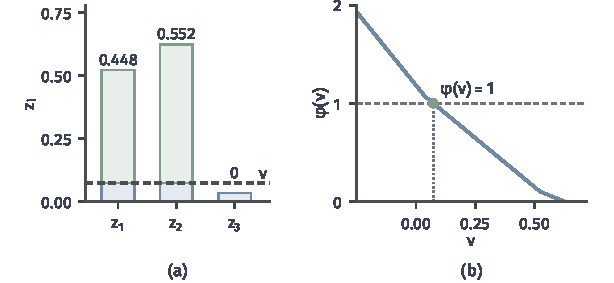
\includegraphics[width=104mm]{figures/05-optimization/06-constrained-optimization/matplotlib/feas-water-level/figure.pdf}
  \caption{单纯形投影的统一阈值，输入$\bm{z}=(0.521875,0.625,0.034375)$。(a)虚线是阈值$\nu$，绿色部分是投影结果，第三个柱子低于阈值，分到$0$。(b)$\varphi(\nu)$是分段线性的递减折线，在每个$z_i$处转折，绿点是$\varphi(\nu)=1$的解$\nu=0.0734375$。}
  \label{fig:feas-water-level}
\end{BookInlineFigure}

\paragraph{求阈值}
把$\bm{z}$从大到小排序为$z_{(1)}\geq\cdots\geq z_{(n)}$。若恰好前$k$个坐标取正，方程~\eqref{eq:feas-simplex-projection}给出
\[
 \nu_k=\frac{1}{k}\Bigl(\sum_{j=1}^kz_{(j)}-1\Bigr).
\]
正确的$k$是满足$z_{(k)}>\nu_k$的最大下标。计算量由排序决定，是$O(n\log n)$。

用图~\ref{fig:feas-water-level}的数据演示。先试$k=3$，$\nu_3=(1.18125-1)/3\approx0.0604$，而最小的坐标$0.034375<0.0604$，不满足要求。再试$k=2$：
\[
 \nu_2=\frac{0.521875+0.625-1}{2}=0.0734375.
\]
这次$z_{(2)}=0.521875>\nu_2$，所以$k=2$，投影是
\[
 \bm{p}=(0.4484375,\;0.5515625,\;0).
\]

\paragraph{投影不是归一化}
把$\bm{z}$除以坐标和也能得到和为一的向量，但这是另一个运算。取$\bm{z}=(0.325,0.625,0.35)$，坐标和$1.3$，归一化得到$(0.25,0.481,0.269)$；投影的阈值是$\nu=0.1$，结果是$(0.225,0.525,0.25)$。投影按相同的量减少各坐标，归一化按相同的比例缩小各坐标。

坐标有负值时差别更大。$\bm{z}'=(0.9,0.5,-0.4)$的坐标和恰好是一，归一化什么也不做，结果仍然不可行。投影取阈值$\nu=0.2$，得到$(0.7,0.3,0)$。图~\ref{fig:feas-projection-cases}(c)在两个坐标的情形画出这种差别：归一化沿过原点的射线回到直线，只有投影沿垂线回来。

\begin{BookInlineFigure}
  \centering
  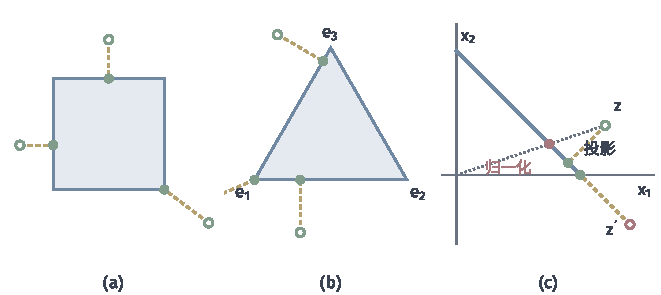
\includegraphics[width=112mm]{figures/05-optimization/06-constrained-optimization/matplotlib/feas-projection-cases/figure.pdf}
  \caption{投影的几何。空心点是输入，实心绿点是投影，黄色虚线是拉回的路径。(a)盒子$[0,1]^2$：逐坐标截断，右下方的点落在角上。(b)单纯形：输入点在三角形所在平面内，可能落到边上，也可能落到顶点。(c)两个坐标的单纯形（蓝线段）：$\bm{z}$的投影与归一化结果（红点，沿过原点的点线）不同；$\bm{z}'$的坐标和已为一，归一化不改变它，它仍然不可行，投影把它送到端点。}
  \label{fig:feas-projection-cases}
\end{BookInlineFigure}

\paragraph{昂贵的投影}
集合复杂时投影没有公式。在$\{\bm{x}:\bm{A}\bm{x}\leq\bm{b}\}$上，式~\eqref{eq:feas-projection}就是一个有$m$个不等式的二次规划，需要用第~\ref{chap:quadratic-conic-programming}章的算法迭代求解。这时外层每一步都包着一个内层优化，内层只能算到有限精度，第~\ref{sec:feas-pgd-step}节会讨论由此带来的误差。

\needspace{6\baselineskip}
\paragraph{变量}
\begin{itemize}
 \item $\bm{x}^{(t)}\in\bm{C}$：当前可行点。
 \item $\bm{g}^{(t)}\in\mathbb{R}^n$：当前梯度。
 \item $\bm{z}^{(t)}\in\mathbb{R}^n$：梯度步的终点，通常不可行。
 \item $\alpha>0$：步长；$\varepsilon>0$与$T$：容差与最大步数。
\end{itemize}

\paragraph{初始化}
取可行起点$\bm{x}^{(0)}\in\bm{C}$，步长$\alpha\leq1/L$，令$t=0$。例中用式~\eqref{eq:feas-running}，取$\alpha=1/L=1/4$，容差$\varepsilon=10^{-3}$，起点和目标值是
\[
 \bm{x}^{(0)}=(0.1,0.2,0.7),\qquad f(\bm{x}^{(0)})=1.25625.
\]

\needspace{6\baselineskip}
\paragraph{每轮更新}
在第$t$轮：
\begin{enumerate}
 \item \textbf{计算梯度步。}令$\bm{z}^{(t)}=\bm{x}^{(t)}-\alpha\bm{g}^{(t)}$。例中第一轮
 \[
  \bm{g}^{(0)}=(-0.9,-1.7,1.4),\qquad \bm{z}^{(0)}=(0.325,0.625,0.35).
 \]
 \item \textbf{投影。}由式~\eqref{eq:feas-simplex-projection}得$\bm{x}^{(t+1)}=P_{\bm{C}}(\bm{z}^{(t)})$。例中第一轮坐标和$1.3$，$k=3$，阈值$\nu=0.1$，于是
 \[
  \bm{x}^{(1)}=(0.225,0.525,0.25),\qquad f(\bm{x}^{(1)})\approx0.38281.
 \]
 \item \textbf{检查停止。}若相邻两点之差的长度除以$\alpha$不超过$\varepsilon$，或$t+1=T$，输出$\bm{x}^{(t+1)}$；否则$t\leftarrow t+1$。例中第一轮这个量约为$2.28$，继续。
\end{enumerate}

例中第二轮，$\bm{g}^{(1)}=(-0.775,-0.4,0.5)$，梯度步终点和投影依次是
\[
 \bm{z}^{(1)}=(0.41875,0.625,0.125),\qquad
 \bm{x}^{(2)}=(0.3625,0.56875,0.06875).
\]
这一轮$\nu=0.05625$，三个坐标仍然为正，$f(\bm{x}^{(2)})\approx0.21426$。

例中第三轮，$\bm{g}^{(2)}=(-0.6375,-0.225,0.1375)$，梯度步终点是图~\ref{fig:feas-water-level}用过的$\bm{z}^{(2)}$。前面已算出$\nu=0.0734375$，第三个坐标被截到零：
\[
 \bm{x}^{(3)}=(0.4484375,0.5515625,0),\qquad f(\bm{x}^{(3)})\approx0.16290.
\]

此后迭代留在底边上。由$x_3=0$和$x_2=1-x_1$代入，每轮的投影化成一维递推
\[
 x_1^{(t+1)}=\tfrac38x_1^{(t)}+\tfrac{5}{16},\qquad t\geq3,
\]
不动点是$x_1=\tfrac12$，误差每轮乘以$\tfrac38$。

第$10$轮的更新量降到容差以下，最终得到$\bm{x}^{(10)}\approx(0.49995,0.50005,0)$。图~\ref{fig:feas-pgd-path}(a)是这条路径，第三步落到活动边之后再也没有离开。

\begin{BookInlineFigure}
  \centering
  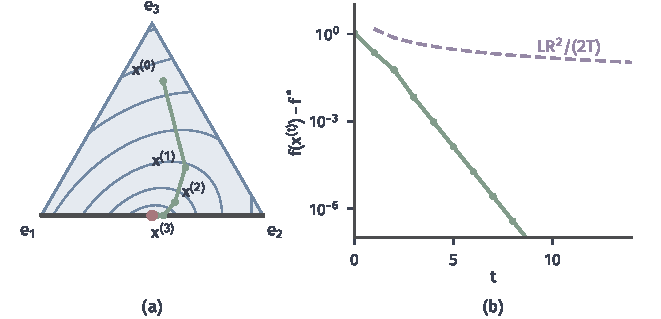
\includegraphics[width=112mm]{figures/05-optimization/06-constrained-optimization/matplotlib/feas-pgd-path/figure.pdf}
  \caption{预算例上的投影梯度法，$\alpha=1/4$，起点$(0.1,0.2,0.7)$。(a)绿色路径在第三步到达活动边（深灰），红点是最优解。(b)绿线是实际目标差，紫色虚线是第~\ref{sec:feas-pgd-step}节证明的上界$LR^2/(2T)$，$R^2=\lVert\bm{x}^{(0)}-\bm{x}^\star\rVert_2^2=0.74$。这个例子强凸，实际收敛比$1/T$快得多。}
  \label{fig:feas-pgd-path}
\end{BookInlineFigure}

\subsection{投影梯度残差}
\label{sec:feas-pgd-residual}

无约束时用$\lVert\nabla f\rVert_2$判断停止。有约束时这把尺子失灵：预算例的最优解处$\nabla f(\bm{x}^\star)=(-\tfrac12,-\tfrac12,0)$并不为零。那么应该用什么量来判断“已经到了”？

\paragraph{残差的定义}
一个点走不动，意思是走一步再投影又回到原地。把这个位移除以步长，单位就和梯度一致。

\begin{definition}[投影梯度残差]
\label{def:feas-residual}
设$\alpha>0$，$\bm{x}\in\bm{C}$。称
\begin{equation}
 \bm{G}_\alpha(\bm{x})=\frac{1}{\alpha}\Bigl[\bm{x}-P_{\bm{C}}\bigl(\bm{x}-\alpha\nabla f(\bm{x})\bigr)\Bigr]
 \label{eq:feas-residual}
\end{equation}
为\term{投影梯度残差}（projected gradient residual）。
\end{definition}

$\bm{C}=\mathbb{R}^n$时投影不起作用，$\bm{G}_\alpha=\nabla f$，所以它是梯度的推广。第~\ref{sec:feas-pgd-projection}节的停止量正是$\lVert\bm{G}_\alpha(\bm{x}^{(t)})\rVert_2$。

\paragraph{残差为零意味着什么}
凸集上的一阶必要条件是下面的\term{变分不等式}（variational inequality）：对可行方向$\bm{y}-\bm{x}$，目标的方向导数不能为负。推导很短：若$\bm{x}$是局部极小点，$\bm{y}\in\bm{C}$，线段$\bm{x}+s(\bm{y}-\bm{x})$在$s\in[0,1]$上可行，所以
\[
 0\leq\lim_{s\downarrow0}\frac{f(\bm{x}+s(\bm{y}-\bm{x}))-f(\bm{x})}{s}=\langle\nabla f(\bm{x}),\bm{y}-\bm{x}\rangle.
\]

\begin{theorem}[残差为零与变分不等式]
\label{thm:feas-residual}
设$\bm{C}$非空闭凸，$f$在$\bm{x}\in\bm{C}$处可微，$\alpha>0$。则$\bm{G}_\alpha(\bm{x})=\bm{0}$当且仅当
\begin{equation}
 \langle\nabla f(\bm{x}),\bm{y}-\bm{x}\rangle\geq0,\quad\forall\bm{y}\in\bm{C}.
 \label{eq:feas-vi}
\end{equation}
若$f$还是凸函数，这又等价于$\bm{x}$是$f$在$\bm{C}$上的全局最优解。
\end{theorem}

\begin{proof}
$\bm{G}_\alpha(\bm{x})=\bm{0}$就是$\bm{x}=P_{\bm{C}}(\bm{x}-\alpha\nabla f(\bm{x}))$。在式~\eqref{eq:feas-projection-vi}中取$\bm{p}=\bm{x}$，$\bm{z}=\bm{x}-\alpha\nabla f(\bm{x})$，这等价于
\[
 \langle-\alpha\nabla f(\bm{x}),\bm{y}-\bm{x}\rangle\leq0,\quad\forall\bm{y}\in\bm{C}.
\]
除以$-\alpha<0$，不等号反向，即得式~\eqref{eq:feas-vi}。

$f$凸时，切平面从下方托住目标，所以
\[
 f(\bm{y})\geq f(\bm{x})+\langle\nabla f(\bm{x}),\bm{y}-\bm{x}\rangle\geq f(\bm{x}),
\]
$\bm{x}$是全局最优解。反方向是前面的一阶必要条件。
\end{proof}

条件~\eqref{eq:feas-vi}里没有$\alpha$，所以残差对某一个$\alpha$为零，就对所有$\alpha>0$为零。残差的大小则随$\alpha$变化，比较时要固定步长。

\paragraph{边界最优点}
现在验证预算例的解。在$\bm{x}^\star=(\tfrac12,\tfrac12,0)$处，对任意$\bm{y}\in\bm{\Delta}$，利用$y_1+y_2=1-y_3$，得到
\[
 \langle\nabla f(\bm{x}^\star),\bm{y}-\bm{x}^\star\rangle
 =-\tfrac12(y_1+y_2)+\tfrac12
 =\tfrac12y_3\geq0.
\]
变分不等式成立，目标凸，所以$\bm{x}^\star$是全局最优解。把它代入式~\eqref{eq:feas-running}，得到
\[
 f^\star=\tfrac12\bigl[\tfrac14+\tfrac{1}{16}\bigr]=\tfrac{5}{32}.
\]

梯度不为零，但它指向的是“出不去”的方向。这就好比一个人靠墙站着，墙外地势更低：坡度不为零，他却走不动。图~\ref{fig:feas-boundary-residual}对比了两个边界点。最优点的梯度步终点垂直于活动边，投影原路拉回。另一个点的梯度步有沿边的分量，投影之后确实前进了。

\begin{BookInlineFigure}
  \centering
  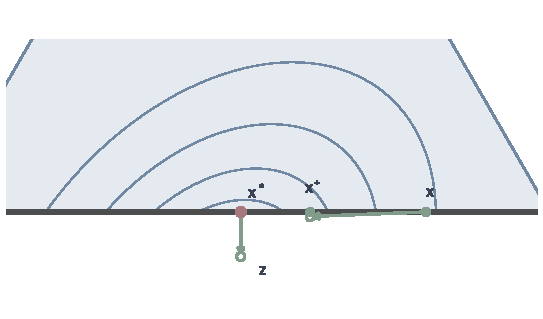
\includegraphics[width=92mm]{figures/05-optimization/06-constrained-optimization/matplotlib/feas-boundary-residual/figure.pdf}
  \caption{残差在活动边上的含义，局部放大底边，$\alpha=1/4$。红点$\bm{x}^\star$处，平面内的梯度步（绿色箭头）垂直离开边，投影回到原处，残差为零而梯度不为零。右侧的$\bm{x}=(0.2,0.8,0)$处，梯度步有沿边分量，投影后到达$\bm{x}^{+}$，残差不为零。}
  \label{fig:feas-boundary-residual}
\end{BookInlineFigure}

\paragraph{非凸时残差只检验驻定}
定理~\ref{thm:feas-residual}的后半句依赖凸性。取一元函数$f(x)=-x^2$，$\bm{C}=[-1,2]$。残差为零的点有三个：$x=-1$、$x=0$、$x=2$。

图~\ref{fig:feas-nonconvex-residual}画出了它们。$x=0$是目标的局部极大点；$x=-1$是约束上的局部极小点，$f=-1$；只有$x=2$是全局最优解，$f=-4$。残差只说明“在一阶意义下走不动”，不区分这三种情况。

\begin{BookInlineFigure}
  \centering
  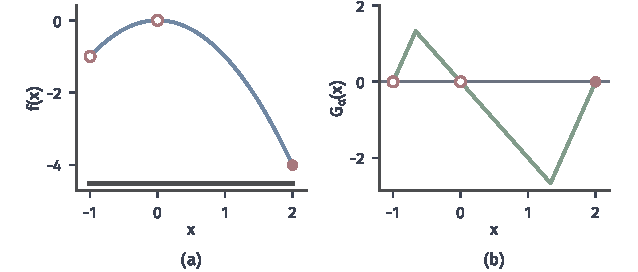
\includegraphics[width=108mm]{figures/05-optimization/06-constrained-optimization/matplotlib/feas-nonconvex-residual/figure.pdf}
  \caption{非凸目标$f(x)=-x^2$，$\bm{C}=[-1,2]$（深灰线）。(a)目标曲线，空心红点是局部极大点$0$和局部极小点$-1$，实心红点是全局最优解$2$。(b)$\alpha=1/4$时的残差$G_\alpha(x)$，在这三个点上都为零。}
  \label{fig:feas-nonconvex-residual}
\end{BookInlineFigure}

\subsection{步长与误差}
\label{sec:feas-pgd-step}

残差为零是目标。迭代是否真的把残差推向零，又需要什么步长？投影只能近似时，保证还剩多少？

\paragraph{单步下降}
投影性质~\eqref{eq:feas-projection-vi}告诉我们投影后的位移仍然是一个下降方向，这是下面所有结论的基础。

\begin{theorem}[投影梯度的单步下降]
\label{thm:feas-pgd-descent}
设$\bm{C}$非空闭凸，$f$在包含$\bm{C}$的开集上可微，且在$\bm{C}$上$L$光滑。对$\bm{x}\in\bm{C}$和$\alpha>0$，记$\bm{x}^{+}$是式~\eqref{eq:feas-pgd}的新点，有
\begin{equation}
 f(\bm{x}^{+})\leq f(\bm{x})-\alpha\Bigl(1-\frac{L\alpha}{2}\Bigr)\lVert\bm{G}_\alpha(\bm{x})\rVert_2^2.
 \label{eq:feas-pgd-descent}
\end{equation}
\end{theorem}

\begin{proof}
在式~\eqref{eq:feas-projection-vi}中取$\bm{z}=\bm{x}-\alpha\nabla f(\bm{x})$，$\bm{p}=\bm{x}^{+}$，$\bm{y}=\bm{x}$，得到
\[
 \langle\bm{x}-\alpha\nabla f(\bm{x})-\bm{x}^{+},\bm{x}-\bm{x}^{+}\rangle\leq0.
\]

整理后得到投影位移与梯度的内积：
\[
 \langle\nabla f(\bm{x}),\bm{x}^{+}-\bm{x}\rangle\leq-\frac1\alpha\lVert\bm{x}^{+}-\bm{x}\rVert_2^2.
\]

$\bm{C}$凸，线段$[\bm{x},\bm{x}^{+}]$在$\bm{C}$中，下降引理可用，于是
\[
 f(\bm{x}^{+})\leq f(\bm{x})+\langle\nabla f(\bm{x}),\bm{x}^{+}-\bm{x}\rangle+\frac L2\lVert\bm{x}^{+}-\bm{x}\rVert_2^2.
\]

把前一式代入，再用$\bm{x}^{+}-\bm{x}=-\alpha\bm{G}_\alpha(\bm{x})$，即得式~\eqref{eq:feas-pgd-descent}。
\end{proof}

只要$0<\alpha<2/L$，式~\eqref{eq:feas-pgd-descent}的括号就是正的，目标严格下降，除非已经驻定。这和无约束的下降估计形式完全相同，只是把梯度换成了残差。

\paragraph{非凸问题}
目标非凸时目标差无从谈起，能评价的是残差。这里需要目标在集合上有下界，否则下降可以无休止地进行。

\begin{theorem}[非凸情形的投影梯度]
\label{thm:feas-pgd-nonconvex}
在定理~\ref{thm:feas-pgd-descent}的条件下，设$f_{\inf}=\inf_{\bm{C}}f>-\infty$，取$\alpha=1/L$，则对$T\geq1$，
\begin{equation}
 \min_{0\leq t<T}\lVert\bm{G}_\alpha(\bm{x}^{(t)})\rVert_2^2\leq\frac{2L\bigl(f(\bm{x}^{(0)})-f_{\inf}\bigr)}{T},
 \label{eq:feas-pgd-nonconvex}
\end{equation}
并且$\{\bm{x}^{(t)}\}$的每个极限点都满足变分不等式~\eqref{eq:feas-vi}。
\end{theorem}

\begin{proof}
由式~\eqref{eq:feas-pgd-descent}，$\alpha=1/L$时
\[
 \frac{1}{2L}\lVert\bm{G}_\alpha(\bm{x}^{(t)})\rVert_2^2\leq f(\bm{x}^{(t)})-f(\bm{x}^{(t+1)}).
\]
对$t=0,\ldots,T-1$求和，右端裂项，并用$f(\bm{x}^{(T)})\geq f_{\inf}$，最小值不超过平均值，即得式~\eqref{eq:feas-pgd-nonconvex}。

级数$\sum_t\lVert\bm{G}_\alpha(\bm{x}^{(t)})\rVert_2^2$收敛，所以残差趋于零。若梯度连续，投影非扩张保证$\bm{G}_\alpha$连续，极限点处残差为零。定理~\ref{thm:feas-residual}给出结论。
\end{proof}

\paragraph{凸问题}
加上凸性和解的存在，可以用目标差衡量。证明的关键是把一步的目标差写成到解距离平方的差，这样求和时能够裂项。

\begin{theorem}[凸情形的投影梯度]
\label{thm:feas-pgd-convex}
在定理~\ref{thm:feas-pgd-descent}的条件下，设$f$在$\bm{C}$上凸，且存在最优解$\bm{x}^\star\in\bm{C}$，取$\alpha=1/L$。则对$T\geq1$，
\begin{equation}
 f(\bm{x}^{(T)})-f^\star\leq\frac{L\lVert\bm{x}^{(0)}-\bm{x}^\star\rVert_2^2}{2T}.
 \label{eq:feas-pgd-convex}
\end{equation}
若$f$还在$\bm{C}$上$\mu$强凸，$\mu>0$，则
\begin{equation}
 \lVert\bm{x}^{(t+1)}-\bm{x}^\star\rVert_2^2\leq\Bigl(1-\frac\mu L\Bigr)\lVert\bm{x}^{(t)}-\bm{x}^\star\rVert_2^2.
 \label{eq:feas-pgd-strong}
\end{equation}
\end{theorem}

\begin{proof}
记$\bm{x}=\bm{x}^{(t)}$，$\bm{x}^{+}=\bm{x}^{(t+1)}$，$\bm{g}=\nabla f(\bm{x})$，$\bm{y}\in\bm{C}$任取。由下降引理和$\mu$强凸的下界（$\mu=0$即凸），得到
\[
 \begin{aligned}
 f(\bm{x}^{+})&\leq f(\bm{x})+\langle\bm{g},\bm{x}^{+}-\bm{x}\rangle+\frac L2\lVert\bm{x}^{+}-\bm{x}\rVert_2^2,\\
 f(\bm{y})&\geq f(\bm{x})+\langle\bm{g},\bm{y}-\bm{x}\rangle+\frac\mu2\lVert\bm{y}-\bm{x}\rVert_2^2.
 \end{aligned}
\]

两式相减，消去$f(\bm{x})$：
\[
 f(\bm{x}^{+})-f(\bm{y})\leq\langle\bm{g},\bm{x}^{+}-\bm{y}\rangle+\frac L2\lVert\bm{x}^{+}-\bm{x}\rVert_2^2-\frac\mu2\lVert\bm{y}-\bm{x}\rVert_2^2.
\]

在式~\eqref{eq:feas-projection-vi}中取$\bm{z}=\bm{x}-\bm{g}/L$，$\bm{p}=\bm{x}^{+}$，整理得
\[
 \langle\bm{g},\bm{x}^{+}-\bm{y}\rangle\leq L\langle\bm{x}-\bm{x}^{+},\bm{x}^{+}-\bm{y}\rangle.
\]

再用恒等式展开$\lVert\bm{x}-\bm{y}\rVert_2^2$，它把内积化成三个距离平方：
\[
 2\langle\bm{x}-\bm{x}^{+},\bm{x}^{+}-\bm{y}\rangle
 =\lVert\bm{x}-\bm{y}\rVert_2^2-\lVert\bm{x}-\bm{x}^{+}\rVert_2^2-\lVert\bm{x}^{+}-\bm{y}\rVert_2^2.
\]

代回去，$\lVert\bm{x}^{+}-\bm{x}\rVert_2^2$的项抵消，得到
\[
 f(\bm{x}^{+})-f(\bm{y})\leq\frac{L-\mu}{2}\lVert\bm{x}-\bm{y}\rVert_2^2-\frac L2\lVert\bm{x}^{+}-\bm{y}\rVert_2^2.
\]

取$\bm{y}=\bm{x}^\star$，左端非负，移项除以$L/2$，就是式~\eqref{eq:feas-pgd-strong}；$\mu=0$时说明到解的距离不增。

$\mu=0$时对$t=0,\ldots,T-1$求和，右端裂项：
\[
 \sum_{t=1}^T\bigl(f(\bm{x}^{(t)})-f^\star\bigr)\leq\frac L2\lVert\bm{x}^{(0)}-\bm{x}^\star\rVert_2^2.
\]
由定理~\ref{thm:feas-pgd-descent}目标逐步下降，最后一项最小，不超过平均值，即得式~\eqref{eq:feas-pgd-convex}。
\end{proof}

预算例中$R^2=0.74$，$L=4$，上界是$1.48/T$，$T=1$时为$1.48$，实际目标差是$0.2266$。强凸的保证给出距离平方每步至少乘以$\tfrac34$。实际到达活动边之后因子是$(\tfrac38)^2\approx0.14$。约束把自由度减到一维，沿边方向$(1,-1,0)$的曲率是$\tfrac52$，比全空间最小的曲率$\mu=1$大。

\paragraph{$L$未知时}
可以用回溯代替固定步长：试探$\alpha$，算出$\bm{x}^{+}$，检查
\[
 f(\bm{x}^{+})\leq f(\bm{x})+\langle\nabla f(\bm{x}),\bm{x}^{+}-\bm{x}\rangle+\frac{1}{2\alpha}\lVert\bm{x}^{+}-\bm{x}\rVert_2^2,
\]
不满足就缩短$\alpha$。上面的证明只用到这个不等式，结论把$L$换成$1/\alpha_{\min}$仍成立。要注意，换一次$\alpha$就要重新投影，集合复杂时这是真实的成本。

\paragraph{近似投影}
投影由内层迭代求出时，输出$\tilde{\bm{x}}^{+}$与真投影有差距。设
\[
 \bigl\lVert\tilde{\bm{x}}^{+}-P_{\bm{C}}(\bm{x}-\alpha\nabla f(\bm{x}))\bigr\rVert_2\leq\varepsilon_t.
\]
这个误差有三种影响，要分别看待。

第一是可行性。输出到$\bm{C}$的距离不超过$\varepsilon_t$，但不一定是零，所以要单独检查原约束的残差。

第二是误差传播。设$f$的光滑、强凸条件在含所有迭代点的凸集上成立，定理~\ref{thm:feas-pgd-convex}说明精确映射把到解的距离至少缩小到$\rho=\sqrt{1-\mu/L}$倍。再加上三角不等式，得到
\begin{equation}
 \lVert\bm{x}^{(t+1)}-\bm{x}^\star\rVert_2\leq\rho\lVert\bm{x}^{(t)}-\bm{x}^\star\rVert_2+\varepsilon_t.
 \label{eq:feas-inexact-recursion}
\end{equation}

$\varepsilon_t\equiv\varepsilon$时展开递推，几何级数求和，距离的上极限不超过$\varepsilon/(1-\rho)$，迭代停在一个与内层精度成比例的范围里。没有强凸时$\rho=1$，上界只能写成$\lVert\bm{x}^{(0)}-\bm{x}^\star\rVert_2+\sum_t\varepsilon_t$，误差必须可求和才不累积。

第三是残差本身。用近似投影算出的残差$\tilde{\bm{G}}_\alpha$满足
\[
 \bigl\lvert\lVert\tilde{\bm{G}}_\alpha\rVert_2-\lVert\bm{G}_\alpha\rVert_2\bigr\rvert\leq\frac{\varepsilon_t}{\alpha}.
\]
所以步长越小，停止量受内层误差的污染越重。图~\ref{fig:feas-inexact-projection}显示了前两种影响。预算例中$\rho\approx0.866$，$1/(1-\rho)\approx7.46$。

\begin{BookInlineFigure}
  \centering
  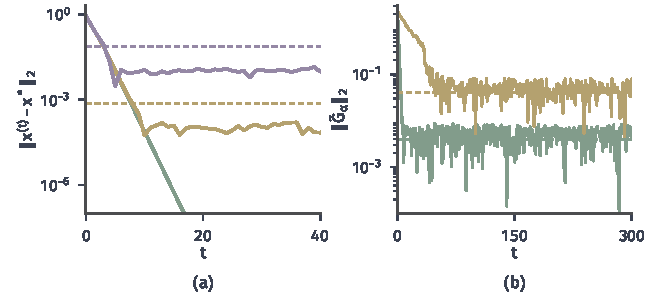
\includegraphics[width=112mm]{figures/05-optimization/06-constrained-optimization/matplotlib/feas-inexact-projection/figure.pdf}
  \caption{近似投影的影响，在每次投影结果上叠加固定种子的随机扰动，长度为$\varepsilon$。(a)到解的距离：绿线是精确投影，黄线$\varepsilon=10^{-4}$，紫线$\varepsilon=10^{-2}$，同色虚线是上界$\varepsilon/(1-\rho)$；距离停在上界之内。(b)$\varepsilon=10^{-3}$时算出的残差：绿线$\alpha=1/4$，黄线$\alpha=1/40$，同色虚线是$\varepsilon/\alpha$；步长小，平台反而高。}
  \label{fig:feas-inexact-projection}
\end{BookInlineFigure}

\paragraph{接近可行不等于接近最优}
内层把“输出离集合多远”算得很准，不能说明外层接近了解。预算例的顶点$\bm{e}_2=(0,1,0)$完全可行，可行误差为零，它的目标差却是$0.625$。可行性和最优性是两件事，都要报告。

\section{条件梯度法（Frank--Wolfe）}
\label{sec:feas-fw}

投影的代价可能很高，而同一个集合上的线性函数却容易最小化。能不能完全不做投影，只靠线性最小化来保持可行？本节回答这个问题：\term{条件梯度法}（conditional gradient method）也称\term{Frank--Wolfe法}（Frank--Wolfe method）\scite{frank1956algorithm}，它要求集合紧，用目标的一阶信息挑选集合的极点，再用凸组合保持可行。

\paragraph{主要思想}
把目标在当前点线性化，$f(\bm{x})+\langle\bm{g},\bm{s}-\bm{x}\rangle$。线性模型没有碗底，无约束时可以降到负无穷，这正是梯度下降要加二次项的原因。现在集合是紧的，线性模型在集合上有最小点，所以可以直接问：只信线性模型的话，集合里哪个点最好？

这个点$\bm{s}^{(t)}$通常在集合的远端，线性模型不能信到那么远。于是不跳过去，只沿连线走一段：
\begin{equation}
 \begin{aligned}
 \bm{s}^{(t)}&\in\argmin_{\bm{s}\in\bm{C}}\langle\bm{g}^{(t)},\bm{s}\rangle,\\
 \bm{x}^{(t+1)}&=\bm{x}^{(t)}+\alpha^{(t)}\bigl(\bm{s}^{(t)}-\bm{x}^{(t)}\bigr),\quad\alpha^{(t)}\in[0,1].
 \end{aligned}
 \label{eq:feas-fw}
\end{equation}

新点是两个可行点的凸组合，所以可行性由$\alpha^{(t)}\in[0,1]$和$\bm{C}$的凸性保证，不需要任何拉回操作。两种方法的次序相反：投影梯度先走一小步再修正，条件梯度先选定目标位置，再决定走多远。

\subsection{线性子问题}
\label{sec:feas-fw-linear}

式~\eqref{eq:feas-fw}的第一行要解一个线性规划。在单纯形上它有闭式解，并且解的形状决定了迭代点的结构。

\paragraph{单纯形上的线性最小化}
对任意$\bm{s}\in\bm{\Delta}$，$\bm{s}$的坐标非负且和为一，$\langle\bm{g},\bm{s}\rangle$是$g_i$的加权平均，所以
\[
 \langle\bm{g},\bm{s}\rangle=\sum_is_ig_i\geq\min_ig_i.
\]
等号在把全部权重放到最小坐标上时取得。因此线性子问题的一个解是顶点
\begin{equation}
 \bm{s}=\bm{e}_{i},\qquad i\in\argmin_kg_k.
 \label{eq:feas-simplex-lmo}
\end{equation}
只需找出梯度的最小分量，计算量是$O(n)$，不用排序。

这个结论在任何紧凸集上都有对应：线性函数的最小值总可以在极点处取到。所以线性子问题的解是集合中结构最简单的点。例如迹为一的半正定矩阵集合的极点是秩一矩阵，线性子问题的解就是$\bm{v}\bm{v}^\top$，其中$\bm{v}$是梯度矩阵最小特征值的单位特征向量。

\paragraph{稀疏表示}
每轮新点等于旧点乘以$1-\alpha^{(t)}$，再给选中的顶点加上权重$\alpha^{(t)}$。若把$\bm{x}^{(t)}$写成顶点的凸组合，权重的更新就是
\begin{equation}
 w_{v}\leftarrow(1-\alpha^{(t)})w_{v},\quad v\neq i;
 \qquad
 w_{i}\leftarrow(1-\alpha^{(t)})w_{i}+\alpha^{(t)}.
 \label{eq:feas-fw-weights}
\end{equation}

从一个顶点出发，每轮至多引入一个新顶点，所以$\bm{x}^{(t)}$至多是$t+1$个顶点的组合。在单纯形上这意味着至多有$t+1$个非零坐标。旧顶点的权重只被等比例缩小，这一点后面会成为问题。

\needspace{6\baselineskip}
\paragraph{变量}
\begin{itemize}
 \item $\bm{x}^{(t)}\in\bm{C}$：当前点；$\bm{g}^{(t)}$：当前梯度。
 \item $\bm{s}^{(t)}\in\bm{C}$：线性子问题的解，这里是顶点。
 \item $w_v$：各活跃顶点的权重，只在需要稀疏表示时保存。
 \item $\alpha^{(t)}\in[0,1]$：组合系数。
\end{itemize}

\paragraph{初始化}
选一个可行点，通常是一个顶点，令$t=0$。例中取$\bm{x}^{(0)}=\bm{e}_3=(0,0,1)$，目标值$f(\bm{x}^{(0)})=2.28125$，组合系数取预定序列
\begin{equation}
 \alpha^{(t)}=\frac{2}{t+2}.
 \label{eq:feas-fw-open-step}
\end{equation}

\needspace{6\baselineskip}
\paragraph{每轮更新}
在第$t$轮：
\begin{enumerate}
 \item \textbf{解线性子问题。}由式~\eqref{eq:feas-simplex-lmo}选顶点。例中第一轮
 \[
  \bm{g}^{(0)}=(-1,-2.5,2),\qquad \bm{s}^{(0)}=\bm{e}_2.
 \]
 \item \textbf{组合。}由式~\eqref{eq:feas-fw}计算新点。例中第一轮$\alpha^{(0)}=1$，新点直接跳到顶点，$\bm{e}_3$的权重变成零：
 \[
  \bm{x}^{(1)}=(0,1,0),\qquad f(\bm{x}^{(1)})=0.78125.
 \]
 \item \textbf{检查停止。}若$t+1=T$，输出$\bm{x}^{(t+1)}$；否则$t\leftarrow t+1$。第~\ref{sec:feas-fw-gap}节会给出可以计算的停止量，例中暂取$T=100$。
\end{enumerate}

例中第二轮，$\bm{g}^{(1)}=(-1,1.5,0)$，选$\bm{e}_1$，$\alpha^{(1)}=\tfrac23$，于是
\[
 \bm{x}^{(2)}=\bigl(\tfrac23,\tfrac13,0\bigr),\qquad f(\bm{x}^{(2)})\approx0.22569.
\]

例中第三轮，$\bm{g}^{(2)}=(-\tfrac13,-\tfrac76,0)$，选$\bm{e}_2$，$\alpha^{(2)}=\tfrac12$，于是
\[
 \bm{x}^{(3)}=\bigl(\tfrac13,\tfrac23,0\bigr),\qquad f(\bm{x}^{(3)})\approx0.22569.
\]

例中第四轮，$\bm{g}^{(3)}=(-\tfrac23,\tfrac16,0)$，选$\bm{e}_1$，$\alpha^{(3)}=\tfrac25$，于是
\[
 \bm{x}^{(4)}=\bigl(\tfrac35,\tfrac25,0\bigr),\qquad f(\bm{x}^{(4)})=0.18125.
\]

规律已经出现：两个顶点轮流被选中，迭代点在解$(\tfrac12,\tfrac12,0)$的两侧来回摆动，幅度慢慢变小。最终在$T=100$得到的点，目标差约为$6.1\times10^{-5}$。

图~\ref{fig:feas-fw-path-weights}画出路径和权重。第一步把起点的权重清零，这是$\alpha^{(0)}=1$的特殊效果。之后的权重在$\bm{e}_1$和$\bm{e}_2$之间来回转移。

\begin{BookInlineFigure}
  \centering
  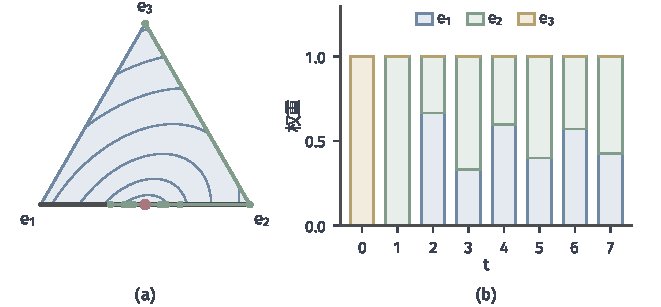
\includegraphics[width=112mm]{figures/05-optimization/06-constrained-optimization/matplotlib/feas-fw-path-weights/figure.pdf}
  \caption{条件梯度法的路径与权重，$\alpha^{(t)}=2/(t+2)$，从顶点$\bm{e}_3$出发。(a)绿色路径先跳到$\bm{e}_2$，然后沿活动边在解（红点）两侧摆动。(b)前$8$个迭代点在三个顶点上的权重，第$t$根柱子的三段高度是$\bm{x}^{(t)}$的三个坐标。}
  \label{fig:feas-fw-path-weights}
\end{BookInlineFigure}

\subsection{步长与可行性}
\label{sec:feas-fw-step}

式~\eqref{eq:feas-fw}中的$\alpha^{(t)}$可以怎样选，不同选法各用到什么信息？

\paragraph{三种规则}
记方向$\bm{d}^{(t)}=\bm{s}^{(t)}-\bm{x}^{(t)}$，用
\begin{equation}
 \Gamma^{(t)}=\langle\bm{g}^{(t)},\bm{x}^{(t)}-\bm{s}^{(t)}\rangle\geq0
 \label{eq:feas-fw-gamma-step}
\end{equation}
表示线性模型沿整条线段预测的下降量。三种规则如下。

\begin{itemize}
 \item \textbf{预定序列。}用式~\eqref{eq:feas-fw-open-step}，不需要函数值，也不需要$L$。
 \item \textbf{线搜索。}$\alpha^{(t)}\in\argmin_{\alpha\in[0,1]}f(\bm{x}^{(t)}+\alpha\bm{d}^{(t)})$，把范围限制在$[0,1]$是为了留在线段上。
 \item \textbf{光滑上界。}最小化下降引理的上界，在$[0,1]$上截断：
\end{itemize}
\begin{equation}
 \alpha^{(t)}=\min\Bigl\{1,\ \frac{\Gamma^{(t)}}{L\lVert\bm{d}^{(t)}\rVert_2^2}\Bigr\}.
 \label{eq:feas-fw-smooth-step}
\end{equation}

三种规则都使$\alpha^{(t)}\in[0,1]$。预定序列在$t\geq0$时取值从$1$递减。线搜索按定义在区间内。光滑上界的分子非负，分母为正（若分母为零，则$\bm{s}^{(t)}=\bm{x}^{(t)}$，已不必移动），再用$\min$截断。

在预算例的第一轮比较这三种规则。方向是$\bm{e}_2-\bm{e}_3=(0,1,-1)$，需要的几个量是
\[
 \Gamma^{(0)}=4.5,\qquad \lVert\bm{d}\rVert_2^2=2,\qquad \bm{d}^\top\bm{H}\bm{d}=6.
\]

二次目标上的精确线搜索是$\Gamma/(\bm{d}^\top\bm{H}\bm{d})$，所以
\[
 \alpha_{\text{预定}}=1,\qquad
 \alpha_{\text{线搜索}}=\tfrac34,\qquad
 \alpha_{\text{上界}}=\tfrac{9}{16}.
\]

对应的目标值分别是$0.78125$、$0.59375$和$0.69922$，图~\ref{fig:feas-fw-step-rules}(a)把这三点标在沿线段的目标曲线上。

\begin{BookInlineFigure}
  \centering
  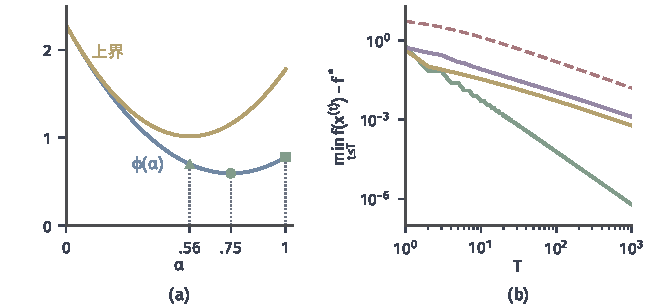
\includegraphics[width=112mm]{figures/05-optimization/06-constrained-optimization/matplotlib/feas-fw-step-rules/figure.pdf}
  \caption{组合系数的三种选法。(a)蓝线是从$\bm{e}_3$到$\bm{e}_2$的线段上的目标$\phi(\alpha)$，黄线是光滑上界，三角、圆点、方块分别是光滑上界、线搜索、预定序列对应的系数。(b)迄今最小目标差：绿线是预定序列，黄线是线搜索，紫线是光滑上界，红色虚线是定理~\ref{thm:feas-fw-rate}的上界$16/(T+2)$。}
  \label{fig:feas-fw-step-rules}
\end{BookInlineFigure}

\paragraph{有限步界}
下面证明目标差的上界，同时把线性子问题解得不准的情形放进去。设$\bm{C}$的直径是$D$，即集合中两点欧氏距离的最大值。证明要用到下一小节将要单独研究的一个事实，这里先在证明中直接用凸性得到。

\begin{theorem}[条件梯度法的有限步界]
\label{thm:feas-fw-rate}
设$\bm{C}$非空紧凸，直径为$D$，$f$在包含$\bm{C}$的开集上可微，在$\bm{C}$上凸且$L$光滑，$\delta\geq0$。设线性子问题的解$\tilde{\bm{s}}^{(t)}\in\bm{C}$满足
\begin{equation}
 \langle\bm{g}^{(t)},\tilde{\bm{s}}^{(t)}\rangle\leq\min_{\bm{s}\in\bm{C}}\langle\bm{g}^{(t)},\bm{s}\rangle+\frac{\delta}{2}\alpha^{(t)}LD^2,
 \label{eq:feas-inexact-lmo}
\end{equation}
并取$\alpha^{(t)}=2/(t+2)$。则对$T\geq1$，
\begin{equation}
 f(\bm{x}^{(T)})-f^\star\leq\frac{2(1+\delta)LD^2}{T+2}.
 \label{eq:feas-fw-rate}
\end{equation}
\end{theorem}

\begin{proof}
记$e_t=f(\bm{x}^{(t)})-f^\star$，$\alpha=\alpha^{(t)}$，$\bm{s}^\ast$是线性子问题的精确解。由下降引理，并用直径$D$放大移动的长度，得到
\[
 e_{t+1}\leq e_t+\alpha\langle\bm{g}^{(t)},\tilde{\bm{s}}^{(t)}-\bm{x}^{(t)}\rangle+\frac{L\alpha^2D^2}{2}.
\]

由式~\eqref{eq:feas-inexact-lmo}，把内积中的$\tilde{\bm{s}}^{(t)}$换成$\bm{s}^\ast$：
\[
 e_{t+1}\leq e_t+\alpha\langle\bm{g}^{(t)},\bm{s}^\ast-\bm{x}^{(t)}\rangle+\frac{(1+\delta)L\alpha^2D^2}{2}.
\]

由凸性，切平面在解处不高于目标，再由$\bm{s}^\ast$在线性模型上最优，得到
\[
 \langle\bm{g}^{(t)},\bm{s}^\ast-\bm{x}^{(t)}\rangle\leq\langle\bm{g}^{(t)},\bm{x}^\star-\bm{x}^{(t)}\rangle\leq-e_t.
\]

记$K=(1+\delta)LD^2$，于是得到递推
\[
 e_{t+1}\leq(1-\alpha^{(t)})e_t+\frac{K(\alpha^{(t)})^2}{2}.
\]

下面对$T$归纳证明$e_T\leq2K/(T+2)$。$t=0$时$\alpha^{(0)}=1$，递推给出$e_1\leq K/2\leq2K/3$。设$e_t\leq2K/(t+2)$，$t\geq1$，代入$\alpha^{(t)}=2/(t+2)$：
\[
 e_{t+1}\leq\frac{t}{t+2}\cdot\frac{2K}{t+2}+\frac{2K}{(t+2)^2}=\frac{2K(t+1)}{(t+2)^2}.
\]

由$(t+1)(t+3)\leq(t+2)^2$，右端不超过$2K/(t+3)$，归纳完成。
\end{proof}

$\delta$的作用是把内层误差与外层步长联系起来：式~\eqref{eq:feas-inexact-lmo}允许的误差随$\alpha^{(t)}$减小，也就是越到后面线性子问题要解得越准。如果误差固定不变，递推中多出常数项$\alpha^{(t)}\varepsilon$，目标差最终停在$\varepsilon$的量级。

线搜索和光滑上界的步长满足同样的上界。两者的新点都不高于在$\alpha=2/(t+2)$处的上界值，所以$\delta=0$时递推不变。第一轮的比较也说明，线搜索每步下降最多，并不代表后面的路径更好：图~\ref{fig:feas-fw-step-rules}(b)中，预定序列在这个例子上反而最快，第~\ref{sec:feas-fw-away}节解释其中的原因。

预算例中$D^2=2$，$L=4$，界~\eqref{eq:feas-fw-rate}是$16/(T+2)$，$T=100$时约为$0.157$，实际目标差约$6\times10^{-5}$。这个界对所有满足条件的问题都成立，所以偏于保守。线搜索的黄线大致按$1/T$下降：解在多面体的边上而不是顶点时，线搜索版本的目标差一般不能比$1/T$快多少，证明需要构造性的下界分析，篇幅较长，读者可查阅Frank--Wolfe方法收敛下界的专门文献。预定序列的绿线约按$1/T^2$下降，这来自两个顶点在解的两侧交替抵消的特殊结构，定理并不提供这样的保证。

\subsection{Frank--Wolfe间隙}
\label{sec:feas-fw-gap}

投影梯度用残差判断停止。条件梯度能不能在不知道$f^\star$的情况下，判断离最优还有多远？线性子问题已经算出了答案。

\paragraph{定义与上界}
式~\eqref{eq:feas-fw-gamma-step}的量可以对任意可行点定义。

\begin{definition}[Frank--Wolfe间隙]
\label{def:feas-fw-gap}
设$\bm{C}$非空紧凸，$f$在$\bm{x}\in\bm{C}$处可微，称
\begin{equation}
 \Gamma(\bm{x})=\max_{\bm{s}\in\bm{C}}\langle\nabla f(\bm{x}),\bm{x}-\bm{s}\rangle
 \label{eq:feas-fw-gap}
\end{equation}
为\term{Frank--Wolfe间隙}（Frank--Wolfe gap）。
\end{definition}

取$\bm{s}=\bm{x}$可知$\Gamma(\bm{x})\geq0$。它的值就是线性子问题的副产品，不需要额外计算：式~\eqref{eq:feas-fw-gamma-step}的$\Gamma^{(t)}$正是$\Gamma(\bm{x}^{(t)})$。

这里没有沿用字母$g$，因为$\bm{g}^{(t)}$已经表示梯度。

\begin{theorem}[间隙上界目标差]
\label{thm:feas-fw-gap}
在定义~\ref{def:feas-fw-gap}的条件下，$\Gamma(\bm{x})=0$当且仅当$\bm{x}$满足变分不等式~\eqref{eq:feas-vi}。若$f$在$\bm{C}$上凸，则
\begin{equation}
 f(\bm{x})-\min_{\bm{C}}f\leq\Gamma(\bm{x}).
 \label{eq:feas-fw-gap-bound}
\end{equation}
\end{theorem}

\begin{proof}
由式~\eqref{eq:feas-fw-gap}，$\Gamma(\bm{x})=0$就是对所有$\bm{s}\in\bm{C}$，$\langle\nabla f(\bm{x}),\bm{x}-\bm{s}\rangle\leq0$，这正是式~\eqref{eq:feas-vi}。

设$\bm{x}^\star$是最优解，它存在，因为$\bm{C}$紧、$f$连续。由凸性和$\Gamma$的定义，
\[
 f(\bm{x})-f(\bm{x}^\star)\leq\langle\nabla f(\bm{x}),\bm{x}-\bm{x}^\star\rangle\leq\Gamma(\bm{x}).
\]
\end{proof}

图~\ref{fig:feas-fw-gap-tangent}(a)在一元情形说明这个不等式。切线在集合上的最低值位于端点$\bm{s}$，凸函数高于切线，所以最优值高于切线的最低值。切线在当前点的高度是$f(\bm{x})$，$\Gamma$就是这段高度差。这和第~\ref{chap:duality}章用下界判断最优的思路相同，线性化给出了一个可计算的下界
\[
 f(\bm{x})-\Gamma(\bm{x})\leq f^\star.
\]

\begin{BookInlineFigure}
  \centering
  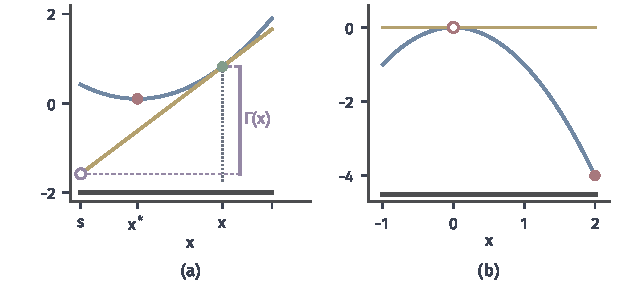
\includegraphics[width=108mm]{figures/05-optimization/06-constrained-optimization/matplotlib/feas-fw-gap-tangent/figure.pdf}
  \caption{间隙的几何。深灰线是可行区间，蓝线是目标，黄线是当前点的切线。(a)凸目标$f(x)=x^2/2+0.1$，$\bm{C}=[-0.8,1.9]$，$x=1.2$：切线在空心紫点处达到区间上的最低值，紫色线段的长度是$\Gamma(x)$，它不小于$f(x)-f^\star$。(b)非凸目标$-x^2$，$\bm{C}=[-1,2]$：局部极大点$x=0$处切线水平，$\Gamma=0$，而全局最优解在$2$。}
  \label{fig:feas-fw-gap-tangent}
\end{BookInlineFigure}

预算例中$\bm{x}^{(3)}=(\tfrac13,\tfrac23,0)$，梯度$(-\tfrac23,\tfrac16,0)$，最小分量是$-\tfrac23$，内积$\langle\bm{g},\bm{x}\rangle=-\tfrac{1}{9}$，于是
\[
 \Gamma(\bm{x}^{(3)})=-\tfrac19+\tfrac23=\tfrac59\approx0.556.
\]
真实目标差约为$0.0694$，不超过间隙。这说明了间隙的特点：可靠但往往偏大。图~\ref{fig:feas-fw-gap-curves}(a)的两条曲线一直保持这种上下关系。

用间隙做停止检验时，可以在每轮计算$\Gamma^{(t)}$，当它不超过容差时输出。把这一步放进第~\ref{sec:feas-fw-linear}节的每轮更新，就得到完整的算法。

\paragraph{非凸目标}
式~\eqref{eq:feas-fw-gap-bound}要用凸性。目标非凸时，$\Gamma=0$只表示一阶驻定，图~\ref{fig:feas-fw-gap-tangent}(b)的局部极大点就是例子。

不过间隙仍能作为进展的度量。取式~\eqref{eq:feas-fw-smooth-step}的步长，把$\lVert\bm{d}\rVert_2$放大为$D$，当$\Gamma\leq LD^2$时一步至少下降$\Gamma^2/(2LD^2)$，否则至少下降$\Gamma/2$。把这些下降量累加，并用$\Delta=f(\bm{x}^{(0)})-\inf_{\bm{C}}f$作为总额，得到
\begin{equation}
 \min_{0\leq t<T}\Gamma(\bm{x}^{(t)})\leq\max\Bigl\{\sqrt{\frac{2LD^2\Delta}{T}},\ \frac{2\Delta}{T}\Bigr\}.
 \label{eq:feas-fw-nonconvex}
\end{equation}
所以驻定度量以$1/\sqrt{T}$的速度减小，和投影残差~\eqref{eq:feas-pgd-nonconvex}开方之后的阶相同。

\paragraph{近似子问题的停止界}
当线性子问题只能近似求解时，设已知误差上界$\varepsilon$：
\[
 \langle\bm{g},\tilde{\bm{s}}\rangle\leq\min_{\bm{s}\in\bm{C}}\langle\bm{g},\bm{s}\rangle+\varepsilon.
\]
用近似解算出来的量记作
\[
 \tilde\Gamma=\langle\bm{g},\bm{x}-\tilde{\bm{s}}\rangle,
\]
它比真实间隙小。把定义和误差条件代入，得到
\begin{equation}
 \tilde\Gamma\leq\Gamma(\bm{x})\leq\tilde\Gamma+\varepsilon.
 \label{eq:feas-inexact-gap}
\end{equation}

$\tilde\Gamma$是真实间隙的下界，单用它停止可能过早。可靠的停止量是$\tilde\Gamma+\varepsilon$，所以必须知道内层求解误差的上界。图~\ref{fig:feas-fw-gap-curves}(b)让内层在最优顶点与次优顶点相差不超过$\varepsilon=0.1$时返回次优顶点，算出的$\tilde\Gamma$甚至可以是负数，而真实间隙一直夹在$\tilde\Gamma$与$\tilde\Gamma+\varepsilon$之间。

\begin{BookInlineFigure}
  \centering
  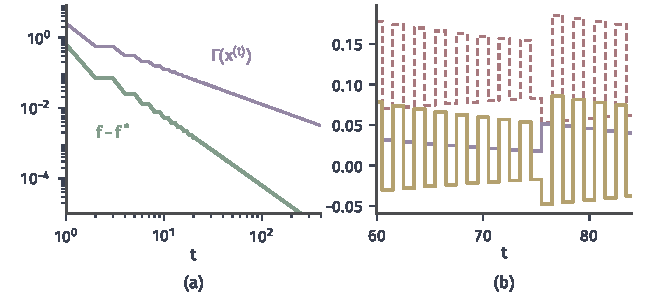
\includegraphics[width=112mm]{figures/05-optimization/06-constrained-optimization/matplotlib/feas-fw-gap-curves/figure.pdf}
  \caption{间隙作为证书，预算例，$\alpha^{(t)}=2/(t+2)$。(a)紫线是$\Gamma(\bm{x}^{(t)})$，绿线是目标差，前者始终在上方。(b)第$60$至$84$轮，内层返回次优顶点时：黄线是算出的$\tilde\Gamma$，紫线是真实间隙$\Gamma$，红色虚线是$\tilde\Gamma+\varepsilon$，$\varepsilon=0.1$。}
  \label{fig:feas-fw-gap-curves}
\end{BookInlineFigure}

\subsection{活跃顶点的调整（补充）}
\label{sec:feas-fw-away}

本小节是补充内容。第~\ref{sec:feas-fw-linear}节留下一个问题：旧顶点的权重只能等比例缩小。如果最优解不用某个顶点，这个顶点的权重永远消不掉，该怎么办？

\paragraph{之字形现象}
用精确线搜索从$\bm{e}_3$出发，第一步$\alpha=\tfrac34$，得到$(0,\tfrac34,\tfrac14)$。第二步$\alpha=\tfrac49$，得到$(\tfrac49,\tfrac{5}{12},\tfrac{5}{36})$。

$\bm{e}_3$的权重每步只乘以$1-\alpha^{(t)}$，线搜索的$\alpha^{(t)}$逐渐变小，第$1000$步第三个坐标仍约为$1.2\times10^{-3}$。图~\ref{fig:feas-fw-away}(a)显示，路径在底边上方反复横跳，既要减小$x_3$，又要调整$x_1,x_2$。这也解释了图~\ref{fig:feas-fw-step-rules}(b)：预定序列的第一步$\alpha^{(0)}=1$恰好把$\bm{e}_3$清零，这个好处只因为起点恰好是要丢弃的顶点，一般问题上不能指望。

\paragraph{远离步}
既然能朝好的顶点走，也应该能从坏的顶点离开。把$\bm{x}$写成活跃顶点集$\bm{S}$上的凸组合，权重$w_{\bm{v}}>0$。\term{远离步}（away step）选出活跃顶点中线性模型最差的一个，沿着背离它的方向走：
\begin{equation}
 \bm{v}^{(t)}\in\argmax_{\bm{v}\in\bm{S}}\langle\bm{g}^{(t)},\bm{v}\rangle,
 \qquad
 \bm{d}=\bm{x}^{(t)}-\bm{v}^{(t)}.
 \label{eq:feas-away}
\end{equation}

新点是$\bm{x}+\gamma\bm{d}$，各权重变成$(1+\gamma)w_{\bm{u}}$，而$\bm{v}^{(t)}$的权重变成$(1+\gamma)w_{\bm{v}}-\gamma$。它必须非负，这给出步长上限
\[
 \gamma\leq\gamma_{\max}=\frac{w_{\bm{v}}}{1-w_{\bm{v}}}.
\]
当$\bm{S}$只有一个顶点时$w_{\bm{v}}=1$，$\gamma_{\max}$无定义，这时不存在远离方向，只走普通的Frank--Wolfe步。取到$\gamma=\gamma_{\max}$时该顶点的权重正好变成零，从活跃集中删除，这称为丢弃步。

\paragraph{成对更新}
另一种做法是把权重直接从最差的活跃顶点搬到最好的顶点。\term{成对步}（pairwise step）取方向$\bm{d}=\bm{s}^{(t)}-\bm{v}^{(t)}$，权重更新是
\[
 w_{\bm{s}}\leftarrow w_{\bm{s}}+\gamma,\qquad
 w_{\bm{v}}\leftarrow w_{\bm{v}}-\gamma,\qquad
 0\leq\gamma\leq w_{\bm{v}}.
\]
其他权重不变，所有权重非负、和为一，所以新点仍是可行的凸组合。

用预算例走一遍，每步用精确线搜索并在上限处截断。第一步只有$\bm{e}_3$活跃，$\bm{s}=\bm{e}_2$，$\gamma=\tfrac34$，到达$(0,\tfrac34,\tfrac14)$。

第二步$\bm{g}=(-1,\tfrac12,\tfrac12)$，$\bm{s}=\bm{e}_1$，$\bm{e}_2,\bm{e}_3$并列最差，取$\bm{v}=\bm{e}_3$。方向$\bm{d}=(1,0,-1)$，精确步长是$1.5/3=\tfrac12$，超过上限$w_{\bm{e}_3}=\tfrac14$，于是截断成丢弃步：
\[
 \bm{x}=\bigl(\tfrac14,\tfrac34,0\bigr).
\]

第三步$\bm{g}=(-\tfrac34,\tfrac12,0)$，$\bm{s}=\bm{e}_1$，$\bm{v}=\bm{e}_2$，方向$(1,-1,0)$，精确步长$\tfrac{5/4}{5}=\tfrac14$，得到
\[
 \bm{x}=\bigl(\tfrac12,\tfrac12,0\bigr).
\]
三步到达最优解，此时$\Gamma=0$。图~\ref{fig:feas-fw-away}对比了这两条路径。

\begin{BookInlineFigure}
  \centering
  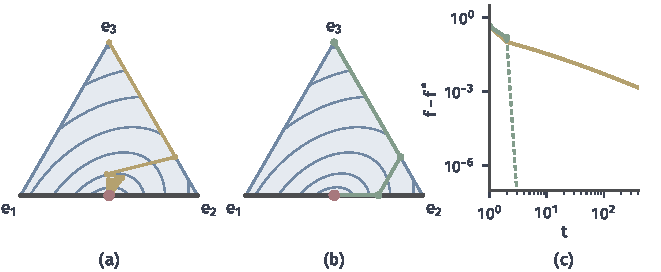
\includegraphics[width=112mm]{figures/05-optimization/06-constrained-optimization/matplotlib/feas-fw-away/figure.pdf}
  \caption{基本流程与成对更新，都用精确线搜索，从$\bm{e}_3$出发。(a)黄色路径是基本的条件梯度法，前$25$步在解上方横跳。(b)绿色路径是成对更新，第二步把$\bm{e}_3$的权重清零，第三步到达解。(c)目标差：黄线是基本流程，绿线是成对更新，第三步目标差为零，虚线表示落到坐标轴下方。}
  \label{fig:feas-fw-away}
\end{BookInlineFigure}

这个三维例子里，到达活动边后问题变成一维二次函数，线搜索一步到位，所以结果格外干净。不能由此推出删除顶点就有线性收敛。这类变体的线性收敛结论依赖目标的曲率、多面体的几何常数（描述顶点相对于面的“尖锐”程度），并要单独计数那些权重被顶到零的步，证明篇幅较长，读者可查阅关于Frank--Wolfe变体线性收敛的专门论文。此外，这些方法要保存活跃顶点及其权重，存储和维护的代价随活跃集增长。

\section{镜像下降}
\label{sec:feas-mirror}

在预算例中，把第三个项目的份额从$0.01$变到$0.02$和从$0.50$变到$0.51$，欧氏距离相同。可是前者把这个项目的份额翻了一倍，后者几乎没有变化。对比例这样的量，有没有一把更合适的尺子？本节回答这个问题：把投影梯度中的欧氏距离换成由凸势函数决定的代价，然后在单纯形上算出具体的公式。

\subsection{Bregman距离}
\label{sec:feas-bregman}

欧氏距离的平方可以看成是$\tfrac12\lVert\bm{x}\rVert_2^2$这个碗与它的切平面之间的高度差。换一只碗，就换了一把尺子。

\paragraph{定义}
设$h$是凸函数，在点$\bm{x}$可微。把$h$在$\bm{x}$处的切平面延伸到$\bm{u}$，势函数实际值高出切平面的量就是我们要的代价。

\begin{definition}[Bregman距离]
\label{def:feas-bregman}
设$h$是凸函数，在$\bm{x}$处可微，$\bm{u}\in\operatorname{dom}h$。称
\begin{equation}
 D_h(\bm{u},\bm{x})=h(\bm{u})-h(\bm{x})-\langle\nabla h(\bm{x}),\bm{u}-\bm{x}\rangle
 \label{eq:feas-bregman}
\end{equation}
为\term{势函数}$h$生成的\term{Bregman距离}（Bregman distance）。
\end{definition}

本节的$h$是势函数，与等式约束无关。由凸性，切平面不高于$h$，所以$D_h(\bm{u},\bm{x})\geq0$；若$h$严格凸，等号只在$\bm{u}=\bm{x}$时成立。

取$h(\bm{x})=\tfrac12\lVert\bm{x}\rVert_2^2$，代入式~\eqref{eq:feas-bregman}，得到
\[
 D_h(\bm{u},\bm{x})=\tfrac12\lVert\bm{u}\rVert_2^2-\tfrac12\lVert\bm{x}\rVert_2^2-\langle\bm{x},\bm{u}-\bm{x}\rangle=\tfrac12\lVert\bm{u}-\bm{x}\rVert_2^2.
\]
这时恰好是欧氏距离平方的一半。

\paragraph{不是真正的距离}
名字里虽有“距离”，$D_h$通常不对称，也不满足三角不等式。图~\ref{fig:feas-bregman-tangent}对比了两种势函数：抛物线上两条竖线段长度相等，$x\ln x$的曲线上两条竖线段长度不同。

\begin{BookInlineFigure}
  \centering
  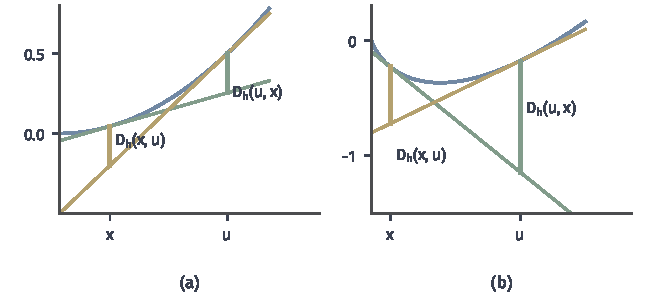
\includegraphics[width=112mm]{figures/05-optimization/06-constrained-optimization/matplotlib/feas-bregman-tangent/figure.pdf}
  \caption{Bregman距离是势函数高出切线的量。蓝线是势函数，绿线和黄线分别是$x$和$u$处的切线，同色竖线段分别是$D_h(u,x)$和$D_h(x,u)$。(a)$h(t)=t^2/2$，两段等长。(b)$h(t)=t\ln t$，$x=0.1$，$u=0.8$，两段不等长。}
  \label{fig:feas-bregman-tangent}
\end{BookInlineFigure}

用一个可手算的例子来看。取$h(\bm{x})=\sum_ix_i\ln x_i$和两个坐标和为一的点
\[
 \bm{u}=(0.5,0.5),\qquad\bm{x}=(0.2,0.8).
\]

这时$D_h(\bm{u},\bm{x})$就是$\sum_iu_i\ln(u_i/x_i)$，推导见第~\ref{sec:feas-entropy}节。代入两种顺序，得到
\[
 D_h(\bm{u},\bm{x})\approx0.2231,\qquad D_h(\bm{x},\bm{u})\approx0.1927.
\]

\paragraph{分析所需的条件}
把$D_h$用到算法里，有三件事要先核对。第一，$\nabla h(\bm{x})$必须存在，所以展开点要在$h$的可微区域内，对熵势就是相对内部。第二，要控制变量移动的大小，需要$h$在某个范数下强凸，也就是$D_h$能从下方控制这个范数的平方。第三，子问题要有解，这要看定义域与集合是否匹配。

图~\ref{fig:feas-kl-balls}比较了这把尺子的“单位球”。在三角形中央，熵势的球接近圆。靠近边界时，球在朝边界的方向被压扁：同样的代价只能让小坐标做很小的绝对变化。

\begin{BookInlineFigure}
  \centering
  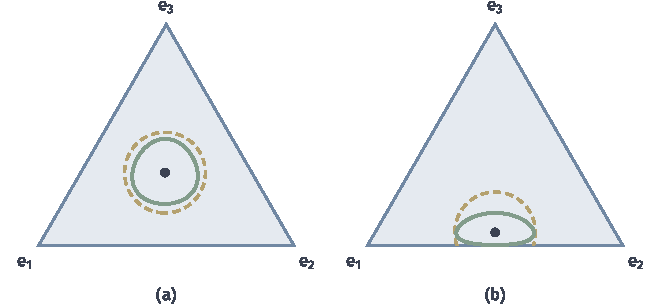
\includegraphics[width=112mm]{figures/05-optimization/06-constrained-optimization/matplotlib/feas-kl-balls/figure.pdf}
  \caption{同一单纯形上两把尺子的等距线。绿色实线是熵势的$\{\bm{u}:D_h(\bm{u},\bm{c})=0.05\}$，黄色虚线是欧氏圆$\{\bm{u}:\tfrac12\lVert\bm{u}-\bm{c}\rVert_2^2=0.025\}$，黑点是中心$\bm{c}$。(a)$\bm{c}\approx(1/3,1/3,1/3)$。(b)$\bm{c}=(0.47,0.47,0.06)$，靠近底边，绿色曲线在朝边的一侧被压扁，黄色圆已越出三角形。}
  \label{fig:feas-kl-balls}
\end{BookInlineFigure}

\subsection{镜像更新}
\label{sec:feas-mirror-update}

有了新尺子，更新公式是什么？它又如何退回熟悉的投影梯度？

\paragraph{主要思想}
投影梯度在$\bm{C}$上最小化线性模型加欧氏距离。把欧氏距离换成$D_h$，就得到\term{镜像下降法}（mirror descent）\scite{beck2003mirror}：
\begin{equation}
 \bm{x}^{(t+1)}\in\argmin_{\bm{x}\in\bm{C}}\Bigl\{\alpha^{(t)}\langle\bm{g}^{(t)},\bm{x}\rangle+D_h(\bm{x},\bm{x}^{(t)})\Bigr\}.
 \label{eq:feas-mirror}
\end{equation}
这里$\bm{g}^{(t)}$可以是当前梯度，也可以是目标非光滑时所选的一个凸次梯度。次梯度的定义见第~\ref{chap:nonsmooth-composite-optimization}章。

$D_h$的作用相当于一根弹簧，把新点拉住，不让它离当前点太远。不同的是，这根弹簧的松紧随位置变化。

\paragraph{完整的计算}
式~\eqref{eq:feas-mirror}可以拆成三步。设$\bm{C}$在$h$的可微区域内，先对$\bm{x}$求驻点。$D_h(\bm{x},\bm{x}^{(t)})$关于$\bm{x}$的梯度是$\nabla h(\bm{x})-\nabla h(\bm{x}^{(t)})$，于是无约束时的驻点$\bm{w}$满足
\begin{equation}
 \nabla h(\bm{w})=\nabla h(\bm{x}^{(t)})-\alpha^{(t)}\bm{g}^{(t)}.
 \label{eq:feas-mirror-dual}
\end{equation}

这说明梯度步不是在变量本身上走，而是在$\nabla h$的值上走。第一步，用$\nabla h$把$\bm{x}^{(t)}$映到梯度空间。第二步，在那里减去$\alpha^{(t)}\bm{g}^{(t)}$。第三步，用$\nabla h$的逆映射取回变量空间，得到$\bm{w}$。

$\bm{w}$可能不在$\bm{C}$中。把式~\eqref{eq:feas-mirror}的目标用式~\eqref{eq:feas-mirror-dual}改写，常数项不影响最小点，于是
\[
 \bm{x}^{(t+1)}=\argmin_{\bm{x}\in\bm{C}}D_h(\bm{x},\bm{w}).
\]
这是按$D_h$度量的投影。图~\ref{fig:feas-mirror-map}把这个往返过程画了出来，“镜像”这个名字指的就是$\nabla h$在两个空间之间的来回映射。

\begin{BookInlineFigure}
  \centering
  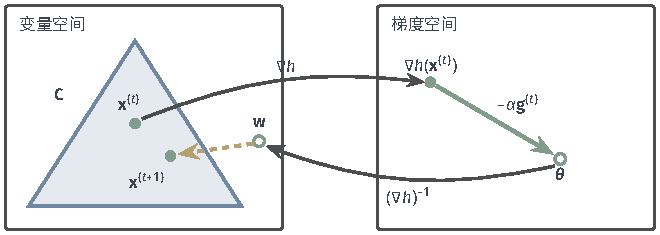
\includegraphics[width=111.74mm]{figures/05-optimization/06-constrained-optimization/tikz/feas-mirror-map/figure.pdf}
  \caption{镜像更新的结构。$\nabla h$把当前点送到梯度空间，绿色箭头在那里减去$\alpha\bm{g}^{(t)}$，逆映射把结果带回变量空间得到$\bm{w}$，黄色虚线按$D_h$投影回集合$\bm{C}$得到$\bm{x}^{(t+1)}$。}
  \label{fig:feas-mirror-map}
\end{BookInlineFigure}

取$h=\tfrac12\lVert\cdot\rVert_2^2$，$\nabla h$是恒等映射，式~\eqref{eq:feas-mirror-dual}给出$\bm{w}=\bm{x}^{(t)}-\alpha^{(t)}\bm{g}^{(t)}$，再做欧氏投影，正是式~\eqref{eq:feas-pgd}。所以投影梯度是镜像下降的特例。

\paragraph{其他势函数要核对的事}
换一个势函数，要分别回答三个问题。解是否存在：若$\bm{C}$紧、$h$连续，子问题有解；否则要检查水平集。解是否唯一：$h$严格凸时唯一。下一步能否继续：$\bm{x}^{(t+1)}$必须落在$h$的可微区域内，否则$\nabla h(\bm{x}^{(t+1)})$不存在，式~\eqref{eq:feas-bregman}无法展开。

第三个问题最容易被忽略。以一元势函数$h(x)=x^{3/2}$（定义域$x\geq0$）为例，导数$\tfrac32\sqrt{x}$在边界保持有限，梯度为正且步长足够大时，子问题的解就落在$x=0$上。这个点在定义域的边界，$h$作为定义域外取$+\infty$的函数在此处不可微。熵势不会发生这种事：它的导数在边界趋于$-\infty$，下一小节会看到迭代被挡在内部。

\subsection{熵势与指数更新}
\label{sec:feas-entropy}

单纯形上的比例变量适合用哪只碗？用\term{熵势}（entropic potential）可以把式~\eqref{eq:feas-mirror}解成闭式，并得到乘法形式的更新。

\paragraph{熵势}
取
\begin{equation}
 h(\bm{x})=\sum_{i=1}^nx_i\ln x_i,\qquad\bm{x}\geq\bm{0},
 \label{eq:feas-entropy}
\end{equation}
并按$0\ln0=0$延拓到坐标为零的边界。$h$在$\bm{x}\geq\bm{0}$上连续，梯度$\nabla h(\bm{x})_i=\ln x_i+1$只在所有坐标为正时存在，所以展开点必须是正向量。

对坐标和都为一的$\bm{u}$和正向量$\bm{x}$，代入式~\eqref{eq:feas-bregman}，线性项中的$\sum_i(u_i-x_i)$等于零，得到
\begin{equation}
 D_h(\bm{u},\bm{x})=\sum_{i=1}^nu_i\ln\frac{u_i}{x_i}.
 \label{eq:feas-kl}
\end{equation}

\paragraph{指数更新}
在$\bm{\Delta}$上解式~\eqref{eq:feas-mirror}。从正向量$\bm{x}^{(t)}$出发，暂时忽略$\bm{x}\geq\bm{0}$，只对等式约束引入乘子$\nu$，对$x_i$求偏导并令其为零：
\[
 \alpha g_i+\ln\frac{x_i}{x_i^{(t)}}+1+\nu=0.
\]

解出$x_i$，常数因子$\mathrm{e}^{-1-\nu}$对所有坐标相同，它由坐标和为一确定，于是
\begin{equation}
 x_i^{(t+1)}=\frac{x_i^{(t)}\exp\bigl(-\alpha g_i\bigr)}{\sum_{j=1}^nx_j^{(t)}\exp\bigl(-\alpha g_j\bigr)}.
 \label{eq:feas-exponential}
\end{equation}

结果每个坐标严格为正，所以被忽略的约束$\bm{x}\geq\bm{0}$确实不活跃，上面的驻点是原子问题的解（目标严格凸，驻点唯一）。下一步的展开点仍是正向量，迭代可以无限进行下去。这种\term{指数更新}（exponentiated update）是乘法的：梯度小的坐标放大，梯度大的坐标缩小，最后归一化。

\paragraph{两个坐标的比较}
设只有两个坐标，$\bm{x}=(0.9,0.1)$，$\bm{g}=(0,1)$，$\alpha=\tfrac12$。投影梯度的梯度步终点是$(0.9,-0.4)$，投影到线段上得到
\[
 \bm{x}^{+}_{\text{投影}}=(1,0).
\]

指数更新先算$(0.9,\;0.1\mathrm{e}^{-1/2})=(0.9,\;0.06065)$，归一化得
\[
 \bm{x}^{+}_{\text{镜像}}\approx(0.9369,0.0631).
\]
投影梯度一步把第二个坐标截到零，镜像更新只把它减小了约$37\%$。

两者的差别随坐标大小变化。两个坐标时投影更新是$x_2^{+}=\max\{x_2-\tfrac12\alpha(g_2-g_1),0\}$，变化量与$x_2$本身无关；镜像更新是乘以一个因子。图~\ref{fig:feas-exp-vs-proj}显示：$x_2=0.5$时两者起步斜率相同；$x_2=0.05$时投影很快归零，镜像更新则按比例缓慢减小。

\begin{BookInlineFigure}
  \centering
  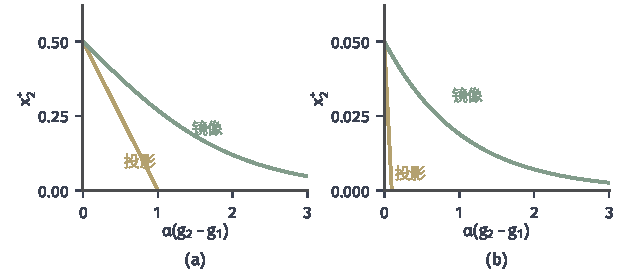
\includegraphics[width=108mm]{figures/05-optimization/06-constrained-optimization/matplotlib/feas-exp-vs-proj/figure.pdf}
  \caption{两个坐标的一步更新，横轴是梯度差乘步长，纵轴是新的$x_2$。黄线是投影更新，绿线是指数更新。(a)$x_2=0.5$，$x_2$较大时两者在起点相切。(b)$x_2=0.05$，投影在横轴$0.1$处归零，指数更新缓慢衰减。}
  \label{fig:feas-exp-vs-proj}
\end{BookInlineFigure}

\needspace{6\baselineskip}
\paragraph{变量}
\begin{itemize}
 \item $\bm{x}^{(t)}\in\bm{\Delta}$：当前点，所有坐标为正。
 \item $\bm{g}^{(t)}$：当前梯度或所选次梯度。
 \item $\bm{w}^{(t)}\in\mathbb{R}^n$：归一化前的正向量。
 \item $\alpha>0$：步长；$T$：总步数。
\end{itemize}

\paragraph{初始化}
取正向量起点，常用均匀分布。例中与投影梯度用同一起点$\bm{x}^{(0)}=(0.1,0.2,0.7)$，步长$\alpha=1/4$，第~\ref{sec:feas-mirror-progress}节说明这个步长的来历。

\needspace{6\baselineskip}
\paragraph{每轮更新}
在第$t$轮：
\begin{enumerate}
 \item \textbf{计算指数因子。}每个坐标乘以指数因子，得到$\bm{w}^{(t)}$。例中第一轮$\bm{g}^{(0)}=(-0.9,-1.7,1.4)$，于是
 \[
  \bm{w}^{(0)}\approx(0.12523,0.30592,0.49328).
 \]
 \item \textbf{归一化。}由式~\eqref{eq:feas-exponential}，把$\bm{w}^{(t)}$除以坐标和得到$\bm{x}^{(t+1)}$。例中第一轮分母约为$0.92443$，于是
 \[
  \bm{x}^{(1)}\approx(0.13547,0.33093,0.53361),\qquad f(\bm{x}^{(1)})\approx0.83140.
 \]
\end{enumerate}

例中第二轮$\bm{g}^{(1)}\approx(-0.8645,-1.1763,1.0672)$，分母约为$1.02087$，于是
\[
 \bm{x}^{(2)}\approx(0.16472,0.43499,0.40030),\qquad f(\bm{x}^{(2)})\approx0.58130.
\]

例中第三轮$\bm{g}^{(2)}\approx(-0.8353,-0.7601,0.8006)$，分母约为$1.05667$，于是
\[
 \bm{x}^{(3)}\approx(0.19208,0.49781,0.31011),\qquad f(\bm{x}^{(3)})\approx0.45489.
\]

运行到$T=60$，目标差约为$6.6\times10^{-5}$，第三个坐标始终为正。最终得到的$\bm{x}^{(60)}$在$x_3$上还有约$1.3\times10^{-4}$的残留量，它每轮大约乘以$0.88$，但不会精确到零。

图~\ref{fig:feas-md-path}将它和投影梯度比较。投影梯度在第$3$步把$x_3$截成零，之后活动集就固定了。镜像下降的路径光滑，$x_3$每轮大约乘以同一个因子。这是一种取舍：投影能识别出活动约束，镜像更新保持稠密的正权重。

\begin{BookInlineFigure}
  \centering
  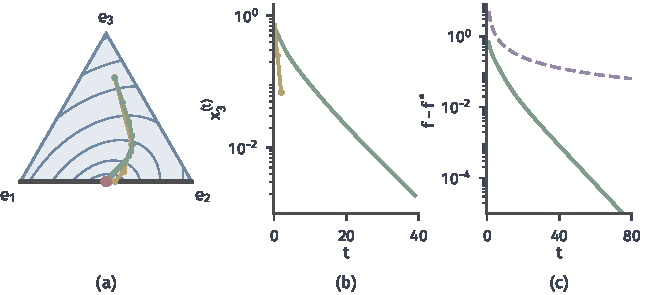
\includegraphics[width=112mm]{figures/05-optimization/06-constrained-optimization/matplotlib/feas-md-path/figure.pdf}
  \caption{预算例上的镜像下降（绿）与投影梯度（黄），步长都是$1/4$，起点$(0.1,0.2,0.7)$。(a)两条路径，镜像下降的路径弯曲着逼近底边。(b)第三个坐标$x_3^{(t)}$（对数轴）：投影梯度第$3$步起为零，从图中消失；镜像下降几何衰减。(c)镜像下降的目标差（绿）与定理~\ref{thm:feas-mirror-smooth}的上界$LD_h(\bm{x}^\star,\bm{x}^{(0)})/T$（紫色虚线）。}
  \label{fig:feas-md-path}
\end{BookInlineFigure}

\subsection{进展与输出}
\label{sec:feas-mirror-progress}

镜像下降的一次更新到底带来了多少进展？目标是否一定下降？答案取决于手上有哪种假设。

\paragraph{三点关系}
分析的工具是下面的引理，它把一次更新转成比较点到两个迭代点的$D_h$之差，求和时可以裂项。

\begin{lemma}[三点关系]
\label{lem:feas-three-point}
设$\bm{C}$闭凸，$h$在开集$\bm{U}$上可微且凸，$\bm{x}\in\bm{U}$，$\bm{x}^{+}$是式~\eqref{eq:feas-mirror}的解，并且$\bm{x}^{+}\in\bm{U}$。则对所有$\bm{u}\in\bm{C}\cap\operatorname{dom}h$，
\begin{equation}
 \alpha\langle\bm{g},\bm{x}^{+}-\bm{u}\rangle\leq D_h(\bm{u},\bm{x})-D_h(\bm{u},\bm{x}^{+})-D_h(\bm{x}^{+},\bm{x}).
 \label{eq:feas-three-point}
\end{equation}
\end{lemma}

\begin{proof}
式~\eqref{eq:feas-mirror}是凸目标在凸集上的最小化，$\bm{x}^{+}$满足变分不等式：
\[
 \bigl\langle\alpha\bm{g}+\nabla h(\bm{x}^{+})-\nabla h(\bm{x}),\ \bm{u}-\bm{x}^{+}\bigr\rangle\geq0.
\]

移项得到
\[
 \alpha\langle\bm{g},\bm{x}^{+}-\bm{u}\rangle\leq\bigl\langle\nabla h(\bm{x}^{+})-\nabla h(\bm{x}),\ \bm{u}-\bm{x}^{+}\bigr\rangle.
\]

把式~\eqref{eq:feas-bregman}的三个距离展开相减，$h(\bm{u})$、$h(\bm{x})$、$h(\bm{x}^{+})$都抵消，剩下的线性项正好是
\[
 D_h(\bm{u},\bm{x})-D_h(\bm{u},\bm{x}^{+})-D_h(\bm{x}^{+},\bm{x})
 =\bigl\langle\nabla h(\bm{x}^{+})-\nabla h(\bm{x}),\ \bm{u}-\bm{x}^{+}\bigr\rangle.
\]
代入上式即得结论。
\end{proof}

\paragraph{次梯度分析}
第一种情形只假设次梯度有界，目标可以不光滑。设$\lVert\cdot\rVert$是某个范数，它的对偶范数是
\[
 \lVert\bm{g}\rVert_{*}=\max_{\lVert\bm{v}\rVert\leq1}\langle\bm{g},\bm{v}\rangle.
\]

\begin{theorem}[镜像下降的平均点界]
\label{thm:feas-mirror-subgrad}
设$\bm{C}$闭凸，$f$在$\bm{C}$上凸，$\bm{g}^{(t)}$是$f$在$\bm{x}^{(t)}$处的次梯度，$\lVert\bm{g}^{(t)}\rVert_{*}\leq G$。设各迭代点都在$h$的可微区域内，且在$\bm{C}$上
\begin{equation}
 D_h(\bm{u},\bm{x})\geq\tfrac12\lVert\bm{u}-\bm{x}\rVert^2.
 \label{eq:feas-h-strong}
\end{equation}
取固定步长$\alpha$，平均点$\bar{\bm{x}}=\frac1T\sum_{t<T}\bm{x}^{(t)}$，则对$\bm{u}\in\bm{C}$，
\begin{equation}
 f(\bar{\bm{x}})-f(\bm{u})\leq\frac{D_h(\bm{u},\bm{x}^{(0)})}{\alpha T}+\frac{\alpha G^2}{2}.
 \label{eq:feas-mirror-rate}
\end{equation}
\end{theorem}

\begin{proof}
记$\bm{x}=\bm{x}^{(t)}$，$\bm{x}^{+}=\bm{x}^{(t+1)}$，$\bm{g}=\bm{g}^{(t)}$。由次梯度不等式，把内积拆成两部分：
\[
 \alpha\bigl(f(\bm{x})-f(\bm{u})\bigr)\leq\alpha\langle\bm{g},\bm{x}^{+}-\bm{u}\rangle+\alpha\langle\bm{g},\bm{x}-\bm{x}^{+}\rangle.
\]

第二项用对偶范数和Young不等式放大，再用$D_h$的强凸下界：
\[
 \alpha\langle\bm{g},\bm{x}-\bm{x}^{+}\rangle\leq\frac{\alpha^2G^2}{2}+\frac12\lVert\bm{x}-\bm{x}^{+}\rVert^2\leq\frac{\alpha^2G^2}{2}+D_h(\bm{x}^{+},\bm{x}).
\]

第一项用引理~\ref{lem:feas-three-point}，$D_h(\bm{x}^{+},\bm{x})$恰好抵消，得到
\[
 \alpha\bigl(f(\bm{x}^{(t)})-f(\bm{u})\bigr)\leq D_h(\bm{u},\bm{x}^{(t)})-D_h(\bm{u},\bm{x}^{(t+1)})+\frac{\alpha^2G^2}{2}.
\]

对$t=0,\ldots,T-1$求和，右端裂项，丢掉末项$D_h\geq0$。两边除以$\alpha T$，再用$f$的凸性把平均值换成$f(\bar{\bm{x}})$，即得结论。
\end{proof}

\paragraph{熵势给出的常数}
在单纯形上，取$\lVert\cdot\rVert=\lVert\cdot\rVert_1$，对偶范数是$\lVert\cdot\rVert_\infty$。熵势满足定理的强凸条件。设$\bm{v}=\bm{u}-\bm{x}$，$\bm{w}$是线段上任一点，$\nabla^2h(\bm{w})=\operatorname{diag}(1/w_i)$，由Cauchy--Schwarz不等式和$\sum_iw_i=1$，
\[
 \bm{v}^\top\nabla^2h(\bm{w})\bm{v}=\sum_i\frac{v_i^2}{w_i}\geq\frac{(\sum_i\lvert v_i\rvert)^2}{\sum_iw_i}=\lVert\bm{v}\rVert_1^2.
\]
由Taylor公式的积分余项，这给出式~\eqref{eq:feas-h-strong}，范数取$\lVert\cdot\rVert_1$。

从均匀分布出发，由式~\eqref{eq:feas-kl}和$\sum_iu_i\ln u_i\leq0$得到$D_h(\bm{u},\bm{x}^{(0)})\leq\ln n$。在式~\eqref{eq:feas-mirror-rate}中取$\alpha=\sqrt{2\ln n/T}/G$，得到
\begin{equation}
 f(\bar{\bm{x}})-f^\star\leq G\sqrt{\frac{2\ln n}{T}},\qquad\lVert\bm{g}^{(t)}\rVert_\infty\leq G.
 \label{eq:feas-entropy-rate}
\end{equation}

投影次梯度法对同一问题的上界要用$\lVert\bm{g}\rVert_2$，而$\lVert\bm{g}\rVert_2$可以大到$\sqrt{n}\,G$。所以梯度稠密时，熵势的上界在维数依赖上小了约$\sqrt{n/\ln n}$倍。这是两个上界的比较，并不保证熵势在每个问题上都更快。

\paragraph{光滑性带来的下降}
第二种情形假设$f$相对于$h$光滑，即存在$L>0$，使$Lh-f$在$\bm{C}$上凸。把凸性写成切平面不等式，它等价于
\begin{equation}
 f(\bm{u})\leq f(\bm{x})+\langle\nabla f(\bm{x}),\bm{u}-\bm{x}\rangle+LD_h(\bm{u},\bm{x}),
 \label{eq:feas-relative-smooth}
\end{equation}
称为\term{相对光滑}（relative smoothness）。$h=\tfrac12\lVert\cdot\rVert_2^2$时它就是下降引理。

预算例满足这个条件。单纯形上$x_i\leq1$，由此
\[
 \bm{v}^\top\nabla^2f\,\bm{v}\leq4\lVert\bm{v}\rVert_2^2\leq4\sum_i\frac{v_i^2}{x_i}=4\,\bm{v}^\top\nabla^2h\,\bm{v},
\]
所以$L=4$可用，这正是取$\alpha=1/4$的依据。

\begin{theorem}[相对光滑下的镜像下降]
\label{thm:feas-mirror-smooth}
设$f$凸可微，满足式~\eqref{eq:feas-relative-smooth}，各迭代点在$h$的可微区域内，取$\alpha=1/L$。则目标逐步下降，
\begin{equation}
 f(\bm{x}^{(t+1)})\leq f(\bm{x}^{(t)})-LD_h(\bm{x}^{(t)},\bm{x}^{(t+1)}),
 \label{eq:feas-mirror-descent}
\end{equation}
并且对$\bm{u}\in\bm{C}$，
\begin{equation}
 f(\bm{x}^{(T)})-f(\bm{u})\leq\frac{LD_h(\bm{u},\bm{x}^{(0)})}{T}.
 \label{eq:feas-mirror-smooth-rate}
\end{equation}
\end{theorem}

\begin{proof}
记$\bm{x}=\bm{x}^{(t)}$，$\bm{x}^{+}=\bm{x}^{(t+1)}$，$\bm{g}=\nabla f(\bm{x})$。由式~\eqref{eq:feas-relative-smooth}，
\[
 f(\bm{x}^{+})\leq f(\bm{x})+\langle\bm{g},\bm{x}^{+}-\bm{x}\rangle+LD_h(\bm{x}^{+},\bm{x}).
\]

在式~\eqref{eq:feas-three-point}中取$\alpha=1/L$，$\bm{u}=\bm{x}$，并用$D_h(\bm{x},\bm{x})=0$，得到
\[
 \langle\bm{g},\bm{x}^{+}-\bm{x}\rangle+LD_h(\bm{x}^{+},\bm{x})\leq-LD_h(\bm{x},\bm{x}^{+}).
\]
两式合起来就是下降式。

再用凸性给出的切平面下界$f(\bm{u})\geq f(\bm{x})+\cdots$，与上面第一式相减，得到
\[
 f(\bm{x}^{+})-f(\bm{u})\leq\langle\bm{g},\bm{x}^{+}-\bm{u}\rangle+LD_h(\bm{x}^{+},\bm{x}).
\]

用式~\eqref{eq:feas-three-point}，右端不超过$L\bigl[D_h(\bm{u},\bm{x})-D_h(\bm{u},\bm{x}^{+})\bigr]$。对$t$求和裂项，再由目标单调，最后一项不超过平均值，即得结论。
\end{proof}

预算例中$D_h(\bm{x}^\star,\bm{x}^{(0)})\approx1.263$，$L=4$，上界约为$5.05/T$，$T=60$时约为$0.084$，实际目标差约$6.6\times10^{-5}$。

\paragraph{目标不一定下降}
定理~\ref{thm:feas-mirror-subgrad}只保证平均点，不保证目标逐步下降，下面的例子说明这是真实的。在$\bm{\Delta}\subset\mathbb{R}^2$上取$f(\bm{x})=\lvert x_1-x_2\rvert$，$\bm{x}=(0.6,0.4)$，次梯度$\bm{g}=(1,-1)$，$\alpha=1$。由式~\eqref{eq:feas-exponential}，
\[
 \bm{x}^{+}\approx(0.1687,0.8313),\qquad f(\bm{x}^{+})\approx0.6626.
\]
目标从$0.2$升到了$0.6626$。次梯度步在不光滑的折点附近可以越过很远，所以输出时应使用平均点，或记录迄今最好的点。表~\ref{tab:feas-mirror-cases}对比了两种分析。

\begin{BookInlineTable}
  \centering
  \caption{镜像下降的两种分析。}
  \label{tab:feas-mirror-cases}
  \begin{tabular}{lll}
   \toprule
   & 次梯度分析 & 相对光滑分析\\
   \midrule
   目标 & 凸，可不光滑 & 凸，相对光滑\\
   势函数 & 按范数强凸 & $Lh-f$凸\\
   步长 & 依$T$或递减 & $1/L$\\
   目标值单调 & 否 & 是\\
   输出 & 平均点 & 最后一点\\
   上界的阶 & $1/\sqrt{T}$ & $1/T$\\
   \bottomrule
  \end{tabular}
\end{BookInlineTable}

\section{广义约化梯度法（GRG）}
\label{sec:feas-grg}

前三节都依赖集合的凸性。圆周$y^2+z^2=1$上，线段离开了约束，投影也不再有前面的性质。这时怎样从一个可行点走到另一个可行点？接下来要弄清：对光滑非线性约束，如何通过局部消元构造下降方向，又如何解方程回到约束上？

\paragraph{问题的形式}
考虑
\begin{equation}
 \min_{\bm{x}}f(\bm{x}),\qquad \bm{c}(\bm{x})=\bm{0},\quad \bm{l}\leq\bm{x}\leq\bm{u},
 \label{eq:feas-grg-problem}
\end{equation}
其中$\bm{c}:\mathbb{R}^n\to\mathbb{R}^p$连续可微，$p<n$。

不等式约束可以化成这个形式。对$g_i(\bm{x})\leq0$引入松弛变量$s_i$，改写成$g_i(\bm{x})+s_i=0$，$s_i\geq0$。例如$x_1^2+x_2^2\leq1$变成$x_1^2+x_2^2+s-1=0$，$s\geq0$。

\paragraph{主要思想}
$p$个方程把$n$个变量中的$p$个绑定了。选出$p$个变量让方程去决定，其余$n-p$个变量自由变动，约束问题就在局部变成只含自由变量的问题。这和线性规划单纯形法中“基变量由非基变量决定”的做法相同，只是这里方程非线性，决定关系是一条曲线，要靠隐函数定理保证存在，靠数值解方程求得。

\term{广义约化梯度法}（generalized reduced gradient method，GRG）依次做三件事：算自由变量上的下降方向，沿这个方向改变自由变量，再解方程把被绑定的变量拉回约束面。

\subsection{变量分块与局部消元}
\label{sec:feas-grg-partition}

选哪些变量由方程决定？选取时要满足什么条件，局部消元才成立？

\paragraph{分块}
把变量分成\term{基本变量}（basic variable）$\bm{y}\in\mathbb{R}^{p}$与\term{非基本变量}（nonbasic variable）$\bm{z}\in\mathbb{R}^{n-p}$，约束写成$\bm{c}(\bm{y},\bm{z})=\bm{0}$。对应地，把当前点的Jacobian矩阵按列分块，记
\begin{equation}
 \bm{B}=\frac{\partial\bm{c}}{\partial\bm{y}}\in\mathbb{R}^{p\times p},
 \qquad
 \bm{N}=\frac{\partial\bm{c}}{\partial\bm{z}}\in\mathbb{R}^{p\times(n-p)}.
 \label{eq:feas-grg-blocks}
\end{equation}

选择分块时有两条要求：$\bm{B}$可逆，基本变量严格位于上下界内。前者保证方程能确定$\bm{y}$，后者保证$\bm{y}$可以朝两边自由调整，用来补偿$\bm{z}$的变化。图~\ref{fig:feas-grg-partition}(a)是这种分块的示意。

\begin{BookInlineFigure}
  \centering
  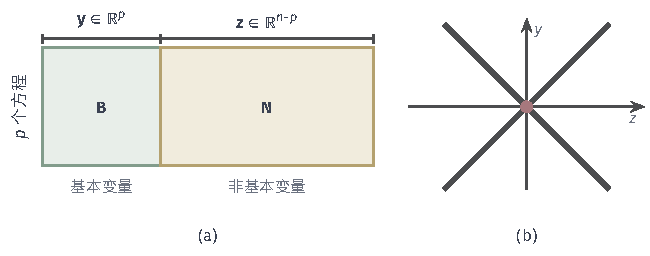
\includegraphics[width=110mm]{figures/05-optimization/06-constrained-optimization/tikz/feas-grg-partition/figure.pdf}
  \caption{局部消元的前提。(a)$p\times n$的Jacobian矩阵按变量分成可逆的方块$\bm{B}$（绿）和其余部分$\bm{N}$（黄）。(b)约束$y^2-z^2=0$的解集是两条相交直线，红点原点处的Jacobian矩阵为零，选哪个变量做基本变量都无法消元。}
  \label{fig:feas-grg-partition}
\end{BookInlineFigure}

\paragraph{局部解出基本变量}
隐函数定理说：若$\bm{c}$连续可微，$\bm{c}(\bm{y}_0,\bm{z}_0)=\bm{0}$，$\bm{B}$在该点可逆，则存在$\bm{z}_0$的邻域和其上唯一的连续可微函数$\bm{y}(\bm{z})$，满足$\bm{y}(\bm{z}_0)=\bm{y}_0$，$\bm{c}(\bm{y}(\bm{z}),\bm{z})=\bm{0}$。定理的证明可参考\BookChapterRef{chap:implicit-inverse-functions}{卷二第22章“隐函数与反函数”}。

把它代入目标，得到只含$\bm{z}$的\term{约化目标}（reduced objective）：
\begin{equation}
 F(\bm{z})=f\bigl(\bm{y}(\bm{z}),\bm{z}\bigr).
 \label{eq:feas-reduced-objective}
\end{equation}
$F$的定义只要求局部能解出$\bm{y}$，并不要求写出显式公式，也不要求全局成立。算法需要$\bm{y}(\bm{z})$的值时，就数值解一次方程。

\paragraph{例子}
本节用下面的问题贯穿：
\begin{equation}
 \min\ y,\qquad y^2+z^2=1.
 \label{eq:feas-circle}
\end{equation}
全局最优解是$(y,z)=(-1,0)$。在点$(\tfrac45,\tfrac35)$，取$y$为基本变量，$B=2y=\tfrac85$可逆，$N=2z=\tfrac65$。在这个点附近$y$由$z$决定，也就是圆周的上半弧：
\[
 y(z)=\sqrt{1-z^2},\qquad F(z)=\sqrt{1-z^2}.
\]
消元只在这一段弧上成立。到$z=\pm1$处$B=0$，上半弧到了头。

\paragraph{分块不存在的情形}
约束在某点的Jacobian矩阵行秩不足时，找不到可逆的$\bm{B}$。图~\ref{fig:feas-grg-partition}(b)的$y^2-z^2=0$在原点就是如此：解集是两条直线的交叉，附近根本不是某一个变量的函数。

基本变量都卡在界上也是一种退化：比如能使$\bm{B}$可逆的列组合都包含位于上下界的变量，这时$\bm{y}$没有双向调整的余地。这些情形需要另行处理，常用的办法有扰动、改用允许退化的换基规则，或换用第~\ref{chap:sequential-quadratic-programming}章的方法。

\subsection{约化梯度与下降方向}
\label{sec:feas-grg-gradient}

有了约化目标，它的梯度怎样算？能不能不必真正解出$\bm{y}(\bm{z})$？

\paragraph{推导}
沿约束面移动时，一阶变化$\mathrm{d}\bm{y}$和$\mathrm{d}\bm{z}$要让$\bm{c}$不变，所以
\[
 \bm{B}\,\mathrm{d}\bm{y}+\bm{N}\,\mathrm{d}\bm{z}=\bm{0}.
\]

解出基本变量的变化：
\begin{equation}
 \mathrm{d}\bm{y}=-\bm{B}^{-1}\bm{N}\,\mathrm{d}\bm{z}.
 \label{eq:feas-grg-dy}
\end{equation}

$\bm{z}$的改变不是孤立的，$\bm{y}$要跟着改变来补偿。目标的一阶变化是两部分之和：
\[
 \mathrm{d}F=\langle\nabla_{\bm{y}}f,\mathrm{d}\bm{y}\rangle+\langle\nabla_{\bm{z}}f,\mathrm{d}\bm{z}\rangle.
\]

代入式~\eqref{eq:feas-grg-dy}，把$\mathrm{d}\bm{z}$提出来，得到\term{约化梯度}（reduced gradient）：
\begin{equation}
 \nabla F=\nabla_{\bm{z}}f-\bm{N}^\top\bm{B}^{-\top}\nabla_{\bm{y}}f.
 \label{eq:feas-reduced-gradient}
\end{equation}

计算时不求逆。先解一个方阵方程$\bm{B}^\top\bm{\pi}=\nabla_{\bm{y}}f$，再算$\nabla F=\nabla_{\bm{z}}f-\bm{N}^\top\bm{\pi}$。$\bm{\pi}$是每单位约束变化的价格。线性约束、线性目标时，这个公式就是第~\ref{chap:simplex-method}章的约化成本。

\paragraph{圆周上的计算}
在式~\eqref{eq:feas-circle}中，$\nabla_yf=1$，$\nabla_zf=0$。在$(\tfrac45,\tfrac35)$，$B=\tfrac85$，$N=\tfrac65$，代入式~\eqref{eq:feas-reduced-gradient}：
\[
 \nabla F=0-\frac65\cdot\frac58\cdot1=-\frac34.
\]

用显式公式核对：$F'(z)=-z/\sqrt{1-z^2}$，在$z=\tfrac35$处正是$-\tfrac34$。

这个数的含义可以这样理解。目标本身不含$z$，$\nabla_zf=0$，单看目标似乎改变$z$没有用处。但$z$增加一点，约束的一阶变化要由$y$补偿：$\mathrm{d}y=-\tfrac34\mathrm{d}z$，而$y$就是目标。所以约化梯度记录的是“经过约束传导之后”的影响。图~\ref{fig:feas-grg-circle}画出了这个补偿三角形，以及约化目标的切线。

\begin{BookInlineFigure}
  \centering
  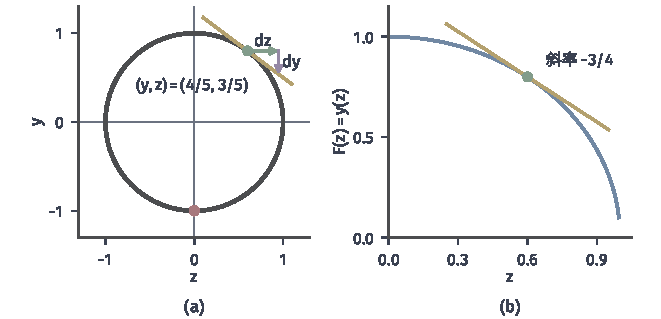
\includegraphics[width=112mm]{figures/05-optimization/06-constrained-optimization/matplotlib/feas-grg-circle/figure.pdf}
  \caption{圆周上的约化梯度。(a)深灰圆是约束，红点是最优解$(y,z)=(-1,0)$，绿点是当前点，黄线是切线；绿色箭头是$\mathrm{d}z$，紫色箭头是基本变量的一阶补偿$\mathrm{d}y=-\tfrac34\mathrm{d}z$。(b)约化目标$F(z)=\sqrt{1-z^2}$，在$z=3/5$处的切线斜率是$-3/4$。}
  \label{fig:feas-grg-circle}
\end{BookInlineFigure}

\paragraph{下降方向}
无界约束时可取$\bm{d}=-\nabla F$。非基本变量有上下界时，顶在界上又想继续往外走的坐标必须置零：
\begin{equation}
 d_j=\begin{cases}
 0,& z_j=l_j\text{ 且 }(\nabla F)_j>0,\\
 0,& z_j=u_j\text{ 且 }(\nabla F)_j<0,\\
 -(\nabla F)_j,& \text{其他}.
 \end{cases}
 \label{eq:feas-grg-direction}
\end{equation}

于是方向导数是
\[
 \langle\nabla F,\bm{d}\rangle=-\sum_{j:\,d_j\neq0}(\nabla F)_j^2.
\]
只要有一个未被置零的坐标，$\bm{d}$就是下降方向。

\subsection{可行恢复与线搜索}
\label{sec:feas-grg-restoration}

沿切向走一步之后点已经离开约束面。怎样回到约束面，又在哪里评价这一步的好坏？

\paragraph{主要思想}
固定候选的$\bm{z}^{+}=\bm{z}+\alpha\bm{d}$，把方程$\bm{c}(\bm{y},\bm{z}^{+})=\bm{0}$看成只含$\bm{y}$的$p$个方程，用Newton法求解，这个过程称为\term{可行恢复}（feasibility restoration）。切向预测$\bm{y}+\alpha\,\mathrm{d}\bm{y}$是一个已经算好的初值。

步长在恢复后的点上判断，比较$F(\bm{z}^{+})$，也就是真实可行点上的目标，而不是切线上的预测值。切线上的目标下降了，不等于回到约束面后依然下降。

\needspace{6\baselineskip}
\paragraph{变量}
\begin{itemize}
 \item $\bm{y}^{(t)}\in\mathbb{R}^p$，$\bm{z}^{(t)}\in\mathbb{R}^{n-p}$：当前基本变量与非基本变量，满足约束。
 \item $\bm{B},\bm{N}$：当前的Jacobian分块，见式~\eqref{eq:feas-grg-blocks}。
 \item $\bm{d}^{(t)}\in\mathbb{R}^{n-p}$：非基本变量的方向。
 \item $\alpha$：试探步长；$c_1\in(0,1)$：Armijo系数；$\varepsilon_c$：约束残差容差；$\varepsilon$：驻定容差。
\end{itemize}

\paragraph{初始化}
需要一个可行点和一个合格的分块。可行点本身可能要另解一个问题，例如最小化$\lVert\bm{c}(\bm{x})\rVert_2^2$。例中从式~\eqref{eq:feas-circle}的可行点出发，取$y$为基本变量，初始试探步长$\alpha=1/4$，$c_1=0.1$，$\varepsilon_c=10^{-10}$：
\[
 (y^{(0)},z^{(0)})=\bigl(\tfrac45,\tfrac35\bigr),\qquad F(z^{(0)})=0.8.
\]

\needspace{6\baselineskip}
\paragraph{每轮更新}
在第$t$轮：
\begin{enumerate}
 \item \textbf{算方向。}由式~\eqref{eq:feas-reduced-gradient}算约化梯度，由式~\eqref{eq:feas-grg-direction}得$\bm{d}^{(t)}$。若$\lVert\bm{d}^{(t)}\rVert_2\leq\varepsilon$，结束并进入第~\ref{sec:feas-grg-basis}节的检验。例中第一轮
 \[
  \nabla F=-0.75,\qquad d^{(0)}=0.75.
 \]

 \item \textbf{切向预测。}令$\bm{z}^{+}=\bm{z}^{(t)}+\alpha\bm{d}^{(t)}$，由式~\eqref{eq:feas-grg-dy}得初值
 \begin{equation}
  \bm{y}_0=\bm{y}^{(t)}-\bm{B}^{-1}\bm{N}\bigl(\bm{z}^{+}-\bm{z}^{(t)}\bigr).
  \label{eq:feas-grg-predict}
 \end{equation}
 例中第一轮
 \[
  z^{+}=0.7875,\qquad y_0=0.659375.
 \]

 \item \textbf{Newton恢复。}反复计算
 \begin{equation}
  \bm{y}_{k+1}=\bm{y}_k-\bm{B}(\bm{y}_k,\bm{z}^{+})^{-1}\bm{c}(\bm{y}_k,\bm{z}^{+}),
  \label{eq:feas-grg-newton}
 \end{equation}
 直到$\lVert\bm{c}\rVert_\infty\leq\varepsilon_c$。例中第一轮的各次结果是
 \[
  \begin{aligned}
  y_0&=0.659375, & c&=5.49\times10^{-2},\\
  y_1&=0.617721, & c&=1.74\times10^{-3},\\
  y_2&=0.616316, & c&=1.97\times10^{-6},\\
  y_3&=0.616315, & c&=2.56\times10^{-12}.
  \end{aligned}
 \]

 \item \textbf{在恢复点上做Armijo检验。}要求
 \[
  F(\bm{z}^{+})\leq F(\bm{z}^{(t)})+c_1\alpha\langle\nabla F,\bm{d}^{(t)}\rangle.
 \]
 通过就接受，否则把$\alpha$减半回到第2步。例中第一轮右端是$0.78594$，$F(z^{+})\approx0.61631$，接受。
\end{enumerate}

图~\ref{fig:feas-grg-recovery}(a)是这一轮的几何。切向预测点（空心）在圆外，Newton迭代沿竖直方向回到圆上。残差的下降呈二次收敛的样子。

\begin{BookInlineFigure}
  \centering
  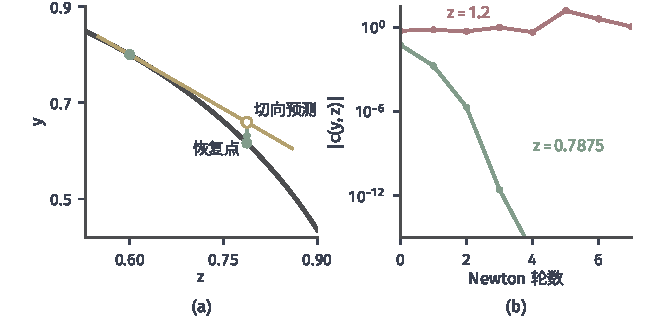
\includegraphics[width=112mm]{figures/05-optimization/06-constrained-optimization/matplotlib/feas-grg-recovery/figure.pdf}
  \caption{可行恢复。(a)从绿点沿切线（黄）走到空心点，固定$z=0.7875$后竖直回到圆周（深灰）。(b)Newton迭代中$\lvert c\rvert$的变化：绿线$z=0.7875$迅速收敛；红线$z=1.2$，方程$y^2+z^2=1$无实解，残差不减小。}
  \label{fig:feas-grg-recovery}
\end{BookInlineFigure}

例中第二轮从$(0.61632,0.7875)$出发，$\nabla F\approx-1.2778$，$d^{(1)}\approx1.2778$。先试$\alpha=\tfrac14$，得$z^{+}\approx1.1069$，超过了$1$，方程没有实解，Newton迭代的残差在几步内不降反升。

于是减半，$\alpha=\tfrac18$，$z^{+}\approx0.94722$，切向预测$y_0\approx0.41223$。Newton迭代依次给出$0.33077$、$0.32074$、$0.32059$，残差由$6.7\times10^{-2}$降到$2.5\times10^{-8}$，再一步达到容差。Armijo检验的右端约为$0.5959$，$F(z^{+})\approx0.32059$，接受：
\[
 (y^{(2)},z^{(2)})\approx(0.32059,0.94722).
\]

例中第三轮$\nabla F\approx-2.955$，方向更陡，而$z$离$1$只剩$0.053$。试探步长要连续减半四次到$\alpha=\tfrac{1}{64}$，得到$z^{+}\approx0.9934$，$y\approx0.1148$。此时$B=2y\approx0.23$已经很小，继续下去方程越来越病态，上半弧也快到头了。下一小节处理这个问题。

\paragraph{恢复失败时}
Newton迭代不收敛有几种可能的原因，处理也不同：步子太大，切向预测离约束面太远，办法是缩短$\alpha$；Jacobian矩阵过时，办法是重新计算；$\bm{B}$接近奇异，办法是换基。

恢复失败和原问题无可行解是两回事。第二轮的$z=1.1069$处方程无解，可是当前点$(0.61632,0.7875)$本身可行。恢复失败只说明这个候选的$\bm{z}^{+}$在这个分块下没有对应的可行点。

\paragraph{恢复容差与Jacobian更新}
恢复的容差要按原约束残差$\lVert\bm{c}\rVert_\infty$设置，不能按Newton步的长度设置。步长短不等于残差小，$\bm{B}$病态时尤其如此。

为了省计算，实现中常常冻结$\bm{B}$，每次Newton迭代只重新算残差。这样收敛变成线性的。第一轮冻结$B=1.6$时，残差依次是
\[
 5.49\times10^{-2},\quad1.08\times10^{-2},\quad2.42\times10^{-3},\quad5.51\times10^{-4},
\]
每次大约缩小$4.5$倍。省下分解矩阵的钱，要用更多的残差计算来付。残差下降变慢时就该更新$\bm{B}$。

\subsection{界约束与换基}
\label{sec:feas-grg-basis}

上面的例子留下两个问题：分块何时必须更换？算法停下来时，怎样判断这个点满足原问题的最优性条件？

\paragraph{一阶必要性}
第~\ref{chap:constrained-optimality}章的KKT条件要求：存在等式乘子和上下界乘子$\bm{\lambda}^{l},\bm{\lambda}^{u}\geq\bm{0}$，使Lagrange函数的梯度为零，并满足互补条件。对问题~\eqref{eq:feas-grg-problem}，这个条件可以用约化梯度来检验。

\begin{theorem}[约化梯度与KKT条件]
\label{thm:feas-grg-kkt}
设$\bm{x}=(\bm{y},\bm{z})$满足式~\eqref{eq:feas-grg-problem}的约束，$\bm{B}$可逆，$\bm{l}_{\bm{y}}<\bm{y}<\bm{u}_{\bm{y}}$。则$\bm{x}$满足KKT条件，当且仅当约化梯度~\eqref{eq:feas-reduced-gradient}的每个分量满足
\begin{equation}
 (\nabla F)_j\begin{cases}
 \geq0,& z_j=l_j,\\
 \leq0,& z_j=u_j,\\
 =0,& l_j<z_j<u_j.
 \end{cases}
 \label{eq:feas-grg-signs}
\end{equation}
此时等式乘子是$\bm{\nu}=-\bm{B}^{-\top}\nabla_{\bm{y}}f$。
\end{theorem}

\begin{proof}
KKT条件的驻定部分按两组变量写开。基本变量严格在界内，互补性使它们的上下界乘子为零，所以
\[
 \nabla_{\bm{y}}f+\bm{B}^\top\bm{\nu}=\bm{0}.
\]
$\bm{B}$可逆，这唯一地确定$\bm{\nu}=-\bm{B}^{-\top}\nabla_{\bm{y}}f$。

非基本变量的驻定条件是
\[
 \nabla_{\bm{z}}f+\bm{N}^\top\bm{\nu}-\bm{\lambda}^{l}_{\bm{z}}+\bm{\lambda}^{u}_{\bm{z}}=\bm{0}.
\]

把$\bm{\nu}$代入，前两项之和正是$\nabla F$，于是
\[
 \nabla F=\bm{\lambda}^{l}_{\bm{z}}-\bm{\lambda}^{u}_{\bm{z}}.
\]

由互补性，$z_j=l_j$时$\lambda^u_j=0$，$(\nabla F)_j=\lambda^l_j\geq0$；$z_j=u_j$时$(\nabla F)_j=-\lambda^u_j\leq0$；在界内时两个乘子都是零，$(\nabla F)_j=0$。反过来，满足式~\eqref{eq:feas-grg-signs}时，按这三种情况取乘子就得到KKT条件。
\end{proof}

用圆周例检验。加上界$z\leq\tfrac35$，点$(\tfrac45,\tfrac35)$处非基本变量在上界，$\nabla F=-\tfrac34\leq0$，符号条件成立。此时$\nu=-\tfrac58$，上界乘子是$\tfrac34$，这个点是带界问题的最优解。若没有这个上界，$\nabla F\neq0$，它就不是驻点。

\paragraph{基本变量碰界}
非基本变量的界由式~\eqref{eq:feas-grg-direction}控制，基本变量是被动的，可能在恢复时越界。例如给圆周例加上$y\geq0.7$，从$(0.8,0.6)$沿$d=0.75$前进。

用切线估计，$y$降到$0.7$的步长是$0.1/0.5625\approx0.178$。但恢复后的点在$z=0.7333$处有$y\approx0.680$，已经越界。所以步长要按恢复后的点限制，真实的碰界点在
\[
 z=\sqrt{1-0.49}\approx0.71414,\qquad\alpha\approx0.1522.
\]

这时$y$到达下界，不再满足“严格在界内”的要求，要做一次换基：$y$变成非基本变量，固定在下界；$z$变成基本变量，$B=2z\approx1.428$可逆。新的约化目标是$F(y)=y$，$\nabla F=1\geq0$，$y$在下界，条件~\eqref{eq:feas-grg-signs}成立。这个点$(0.7,0.71414)$就是带界问题的最优解。

\paragraph{基矩阵病态时换基}
即使没有碰界，$\bm{B}$接近奇异也要换基。上一小节例子的第三轮已经看到：$\lvert B\rvert$变小，约化梯度变陡，步长被压得很短。

一个简单的规则是每轮选取主元较大的变量做基本变量。圆周例只有一个方程，两列分别是$2y$和$2z$，当$\lvert y\rvert<\lvert z\rvert$时让$z$做基本变量。多个方程时，这相当于带列主元的矩阵分解选取一组条件数较好的列。图~\ref{fig:feas-grg-basis}从$(0.8,0.6)$出发，取固定步长$\alpha=1/4$。第二轮起$\lvert y\rvert<\lvert z\rvert$，基本变量换成$z$，新的约化目标$F(y)=y$的梯度是$1$，迭代沿圆周平稳越过$(y,z)=(0,1)$。等到$\lvert z\rvert<\lvert y\rvert$再换回$y$，最后收敛到$(-1,0)$。

\begin{BookInlineFigure}
  \centering
  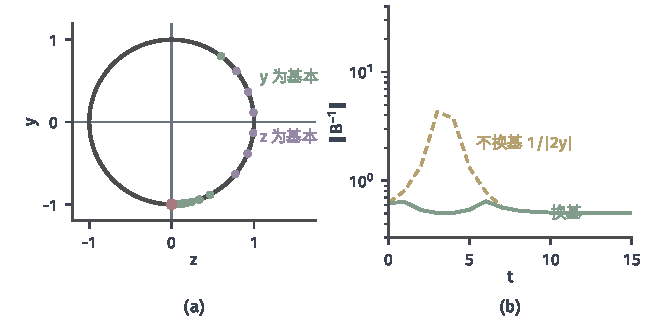
\includegraphics[width=112mm]{figures/05-optimization/06-constrained-optimization/matplotlib/feas-grg-basis/figure.pdf}
  \caption{换基的效果，问题~\eqref{eq:feas-circle}，从$(0.8,0.6)$出发，步长$1/4$。(a)迭代点的颜色表示当轮的基本变量：绿色为$y$，紫色为$z$，红点是最优解。(b)沿同一路径的$\lVert\bm{B}^{-1}\rVert$：黄色虚线是始终以$y$为基本变量时的$1/\lvert2y\rvert$，路径经过$y\approx0$附近时急剧增大；绿线是每轮换基后的值，保持有界。}
  \label{fig:feas-grg-basis}
\end{BookInlineFigure}

\paragraph{运行中要监测什么}
GRG实现要持续监测三类量：$\bm{B}$的条件数，太大就换基；原始可行性$\lVert\bm{c}(\bm{x})\rVert_\infty$和界的违反量；KKT残差，也就是式~\eqref{eq:feas-grg-signs}的违反程度。

\paragraph{每步可行不等于全局最优}
局部表示、可行恢复和换基都有条件，任何一个失败，算法就要改变动作。即使全部成功，得到的也只是满足一阶条件的点。在圆周例中，点$(y,z)=(1,0)$的约化梯度为零，它满足KKT条件，却是目标的最大点。从恰好这一点出发，方法不会移动。约束非凸时，每步可行和目标下降都推不出全局最优。

\section{方法比较}
\label{sec:feas-compare}

前面四种方法该怎样选？本节先按集合结构筛选，再谈成本。比较的前提是同一个问题确实满足所比较方法的条件，并且用相同的可行精度和相同的最优性度量。

\paragraph{先看集合}
选择的第一步是问集合支持什么运算。闭凸集合上可以选投影、线性最小化或Bregman子问题；光滑非线性等式约束只有GRG的局部消元和解方程这条路，前三种方法的保证不适用。反过来，单纯形这样的简单集合也用不着GRG。把适用集合不同的方法排成统一的优劣次序没有意义。

\paragraph{同一问题上的比较}
三种闭凸方法都能解预算例。图~\ref{fig:feas-compare}(a)显示投影梯度最快，因为投影的代价在单纯形上很低，解又落在一条边上，活动集识别后就是一维问题。

图~\ref{fig:feas-compare}(b)换成高维单纯形上的最小二乘问题，看解的稀疏性。条件梯度的非零元个数从一开始缓慢增长，始终很少；投影梯度从稠密起点迅速截断；镜像下降一直保持全部为正。条件梯度的稀疏只是说输出的表示短，并不说明它更准确。

\begin{BookInlineFigure}
  \centering
  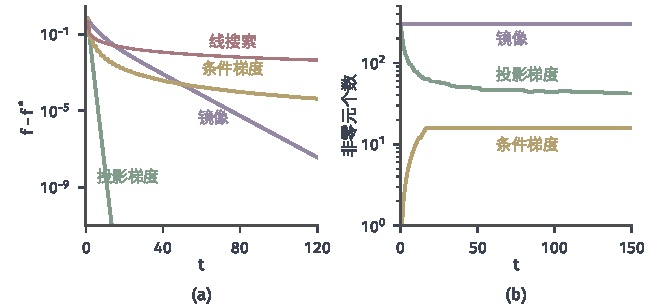
\includegraphics[width=112mm]{figures/05-optimization/06-constrained-optimization/matplotlib/feas-compare/figure.pdf}
  \caption{同一单纯形问题上的比较。(a)预算例的迄今最小目标差：绿线投影梯度，紫线镜像下降，黄线条件梯度（预定序列），红线条件梯度（线搜索）。(b)$n=300$的单纯形最小二乘，随机矩阵$\bm{A}\in\mathbb{R}^{60\times300}$（种子固定），绿线投影梯度和紫线镜像下降从均匀分布出发，黄线条件梯度从一个顶点出发，纵轴是非零元个数。}
  \label{fig:feas-compare}
\end{BookInlineFigure}

表~\ref{tab:feas-compare}归纳了单纯形上每轮的成本和结构。总成本是每轮成本乘以达到相同精度所需的轮数，只看其中一个因子会得出错误的结论。

\begin{BookInlineTable}
  \centering
  \caption{$n$维单纯形上三种方法每轮的额外运算（梯度计算另计）。}
  \label{tab:feas-compare}
  \begin{tabular}{llll}
   \toprule
   方法 & 额外运算 & 输出结构 & 活动约束\\
   \midrule
   投影梯度 & 排序，$O(n\log n)$ & 可稀疏 & 有限步后常被识别\\
   条件梯度 & 找最小分量，$O(n)$ & 顶点的短组合 & 基本流程难以识别\\
   镜像下降 & 乘法与归一化，$O(n)$ & 全部为正 & 不精确识别\\
   \bottomrule
  \end{tabular}
\end{BookInlineTable}

\subsection{内层精度}
\label{sec:feas-compare-inner}

每种方法的子问题都可能只能近似求解。这些内层误差分别影响哪里，又该解到多准？

\paragraph{误差进入的位置}
表~\ref{tab:feas-inner}按方法列出内层误差的去向。投影和GRG的恢复直接影响可行性，线性最小化的误差只影响下降和证书，因为不精确的顶点仍在集合内。

\begin{BookInlineTable}
  \centering
  \caption{内层误差的影响。}
  \label{tab:feas-inner}
  \begin{tabular}{llll}
   \toprule
   内层计算 & 可行性 & 下降 & 停止检验\\
   \midrule
   投影 & 可能略不可行 & 式~\eqref{eq:feas-inexact-recursion} & 残差误差$\varepsilon/\alpha$\\
   线性最小化 & 不受影响 & 式~\eqref{eq:feas-inexact-lmo} & 间隙加$\varepsilon$\\
   镜像子问题 & 视解法而定 & 三点关系多余项 & 同步记录误差\\
   GRG恢复 & 残差至多$\varepsilon_c$ & $F$的值有误差 & 须检查$\bm{c}$\\
   \bottomrule
  \end{tabular}
\end{BookInlineTable}

熵势在单纯形上的子问题有闭式解，归一化的舍入误差可以忽略。一般的集合上，镜像子问题也要迭代求解，并且三点关系~\eqref{eq:feas-three-point}多出误差项，处理方式和近似投影类似。

\paragraph{按外层精度安排内层}
外层离解还远时，把内层解到很高的精度是浪费；外层接近收敛时，内层误差又会成为瓶颈。前面的递推说明了这一点：式~\eqref{eq:feas-inexact-lmo}让线性最小化的容差随$\alpha^{(t)}$减小，式~\eqref{eq:feas-inexact-recursion}说明投影容差决定了误差的平台。常用做法是把内层容差设成外层当前残差的一个比例。

GRG的恢复容差则有一个硬性的下限要求：它决定了输出点的可行程度，至少要达到最终要求的约束精度。

\paragraph{成本要算全}
GRG每轮的成本不只是外层更新，要把下面各项都算进去：
\begin{itemize}
 \item 线搜索中重复的恢复，每次试探步长都要解一次非线性方程；
 \item 每次恢复中的Newton迭代，各需一次约束计算和一次线性方程求解；
 \item Jacobian矩阵的更新与$\bm{B}$的分解，稠密时分解约需$p^3$量级的运算；
 \item 换基之后的重新分解或分解修正。
\end{itemize}

上面圆周例的第三轮就要试探五个步长，其中四个失败或被拒绝，这些计算都要计入总成本。投影梯度的回溯同样要计入重复投影的次数。比较方法时，统计的是这些基本运算的总次数，而不是外层轮数。

\subsection{结果检验}
\label{sec:feas-compare-check}

算法停下来之后，应该报告什么数字来证明结果可用？

\paragraph{凸问题}
凸问题可以报告目标差的上界。条件梯度的间隙$\Gamma$直接就是这样的上界。单纯形上计算$\Gamma$只要$O(n)$，投影梯度或镜像下降也可以顺便算一个间隙作为证书。

没有线性最小化可用时，投影残差也能给出上界。在定理~\ref{thm:feas-pgd-convex}的证明中取$\mu=0$，$\alpha=1/L$，$\bm{y}=\bm{x}^\star$，由内积的上界和残差的定义，得到
\begin{equation}
 f(\bm{x}^{+})-f^\star\leq\lVert\bm{G}_\alpha(\bm{x})\rVert_2\lVert\bm{x}^{+}-\bm{x}^\star\rVert_2+\frac{1}{2L}\lVert\bm{G}_\alpha(\bm{x})\rVert_2^2.
 \label{eq:feas-residual-gap}
\end{equation}
这需要知道到解的距离的上界，比如集合的直径，否则残差小不能换算成目标差小。

\paragraph{非凸光滑问题}
目标非凸时报告驻定度量，$\lVert\bm{G}_\alpha\rVert_2$或$\Gamma$都可以，同时要说明步长，并明确它只检验一阶条件。

\paragraph{GRG}
GRG的报告必须回到原问题的形式：$\lVert\bm{c}(\bm{x})\rVert_\infty$、界的违反量、以及完整的KKT残差。只看约化梯度的范数是不够的。在圆周例的不可行点$(y,z)=(2,0)$上，公式~\eqref{eq:feas-reduced-gradient}算出$\nabla F=0$，而约束残差是$3$。约化梯度的含义依赖于“当前点在约束面上”这个前提。

\paragraph{随机方向}
大规模时梯度常常用随机估计代替。第~\ref{chap:stochastic-gradient-methods}章的分析依赖更新对噪声是线性的，这样条件期望可以直接进入更新。投影和指数映射都是非线性的，期望不能穿过去。

取$\bm{C}=[0,1]$，$x=0$，随机梯度等概率取$\pm1$，期望是零。精确梯度的投影更新留在原地，而随机更新的期望是
\[
 \mathbb{E}\bigl[P_{\bm{C}}(x-\alpha\tilde g)\bigr]=\tfrac12\alpha+\tfrac12\cdot0=\tfrac\alpha2\neq0.
\]

指数映射也是如此：
\[
 \mathbb{E}\bigl[\exp(-\alpha\tilde g)\bigr]=\cosh\alpha>1=\exp\bigl(-\alpha\,\mathbb{E}[\tilde g]\bigr).
\]

所以把随机方向接入投影或镜像更新时，要在变分不等式或三点关系那一层使用条件期望，也就是对内积取期望，然后单独控制噪声带来的二次项，不能把噪声当成在映射之外平均掉。

\section{本章小结}
\label{sec:feas-summary}

本章的问题是怎样让每个迭代点满足原约束，以及保持或恢复可行性要花多少计算。预算例给出了同一问题上的对比，圆周例说明了凸集之外的情形。

投影梯度把梯度步拉回最近点，残差$\bm{G}_\alpha$为零等价于变分不等式，$L$光滑时目标差有$1/T$的界，强凸时距离线性收缩。条件梯度只用线性最小化，靠凸组合保持可行，产生顶点的短组合，间隙$\Gamma$在凸问题上上界目标差。镜像下降把欧氏距离换成Bregman距离，在单纯形上给出保持正性的指数更新；一般次梯度分析针对平均点，只有相对光滑时目标才逐步下降。

GRG面向光滑非线性约束，通过可逆的基矩阵局部消元，按约化梯度移动非基本变量，再解方程恢复基本变量，碰界或病态时换基。它依赖的是局部可解性，与前三种方法的闭凸集假设不同，两边的保证不能互相借用。

各种方法都要分别检查原约束误差和合适的最优性残差。内层投影、线性最小化或恢复不精确时，误差要进入递推和停止检验。可行迭代还需要一个可行的起点，这个起点本身有时也要专门构造。

